%=========================================================================
%===============================================================================

\chapter{Úvod}
Odpovídání na otázky (QA) je dobře prozkoumaný a~populární úkol z~oblasti zpracování přirozeného jazyka (NLP). Využití kolem nás, v~běžném životě, můžeme vidět třeba u~vyhledávacích nástrojů, komunikačních agentů nebo hlasových asistentů. Má také potenciál jako budoucnost získávání informací.\par 
Výzkum se v~dané oblasti soustředí na metody strojového učení pro extrakci odpovědi na otázku ze~získaného kontextu. Kromě porozumění textu jsou v~oblasti důležité také metody pro zhodnocení relevance dokumentů, používané všemi vyhledávacími nástroji, a~v~neposlední řadě také techniky zpracování textu.\par
Pro češtinu je množství a velikost dostupných datových sad oproti angličtině menší, a~je tak obtížné dosáhnout podobných výsledků, jako u~jazyků s~mnoha zdroji (angličtina, němčina, francouzština, \dots). Obzvlášť v~kontextu toho, že pro většinu úkolů na poli porozumění textu se v~posledních letech nejlépe osvědčily velké modely předtrénované na velmi rozsáhlých korpusech textu. Ty pro češtinu prozatím bohužel nejsou ve stejné kvalitě dostupné. Čeština na tom ale není tak špatně. Má rozsáhlou Wikipedii, existují pro ni tedy vícejazyčné modely. Výzkum v oblasti její morfologie a strojového překladu je na výborné úrovni. Jsou pro ni dostupné i kvalitní nástroje pro zpracování textu.\par \smallskip

Cílem práce je vytvořit QA systém, který by byl s pomocí české Wikipedie úspěšný v odpovídání na otázky, ověřit jej na testovací datové sadě SQAD v3.0, porovnat s existujícími řešeními a položit základ pro další podobné systémy nad otevřenou doménou (open-domain).\par \smallskip
V~této práci experimentuji se dvěma přístupy. První využívá pro extrakci odpovědi vícejazyčný model BERT. Druhý pak anglický model ALBERT, pro který jsou získané pasáže textu s otázkou strojově překládány. Kromě metod pro extrakci odpovědi rozebírám  v~práci možnosti řazení dokumentů dle jejich relevance k~otázce.\par

Nejprve jsou v~kapitole~\ref{text_processing} popsány metody pro zpracování a reprezentaci textu. Kapitola \ref{language_comprehension} se zabývá popisem neuronových sítí pro porozumění textu a~extrakci odpovědi. Popsány jsou moderní architektury a~modely použité v~práci. V~kapitole \ref{available_datasets} jsou poté prozkoumány datové sady vhodné pro trénink a~vyhodnocení výsledného systému. Následuje kapitola \ref{chapter:design_}, kde je prezentován návrh systému a přehled již existujících. Kapitola \ref{chapter:implementace} je popisem implementace systému, který je postaven na zmíněných postupech, včetně popisu použitých technologií pro jeho realizaci. Zmíněna je také tvorba demonstrační aplikace -- \href{http://r2d2.fit.vutbr.cz/.cs}{r2d2.fit.vutbr.cz/.cs}. V~kapitole \ref{system_evaluation} je výsledný systém vyhodnocen s~použitím standardních metrik a porovnán se současným stavem, tedy podobnými systémy, které slouží ke stejnému účelu.

%=========================================================================
%===============================================================================

\chapter{Reprezentace slov a~zpracování textu}
\label{text_processing}

Předtím, než se práce dostane k vysvětlení poměrně složitých jazykových modelů a~hodnotících funkcí, je v~této kapitole vysvětleno pár základních pojmů a~technik pro zpracování a reprezentaci textu.\par 
Počítač lidské řeči na elementární úrovni příliš nerozumí. Proto musíme nejdříve porozumět tomu, s~jakou reprezentací slov moderní jazykové modely pracují a~do jaké podoby je nutno zdrojový text dostat. Vysvětleny jsou tedy termíny související s~reprezentací slov pomocí vektorů, neboli \uv{word embeddings} a~tokenizace textu.\par 
Také je důležité popsat způsoby zpracování textů a~slov na jejich morfologické úrovni. Tato úloha je na pomezí informatiky a~lingvistiky a~používají se pro ni speciální nástroje. Použité techniky jako lemmatizace a~odstranění stop-slov zajistí optimální funkčnost některých použitých algoritmů.\par
Po přečtení kapitoly by měl být čtenář teoreticky vybaven pro pochopení konceptů vysvětlených v~kapitolách \ref{language_comprehension} a~\ref{document_indexing}, které na zde popsaných technologiích staví a~částečně se s~nimi překrývají.

%=========================================================================
\section{Reprezentace slov}
\label{reprezentace_slov}
Jak už bylo řečeno, je složité pracovat s~textem v~takové podobě, na jakou jsou lidé zvyklí. Počítač v~ní nedokáže vidět důležité sémantické souvislosti, které jsou pro přirozený jazyk tak důležité. Musíme tedy z~textu a~slov v~něm získat nějakou matematickou reprezentaci, která je počítači bližší a~se kterou dokáží dále nakládat např. modely umělých neuronových sítí. \par
Pro takovou reprezentaci jsou nejpoužívanější vektory pevně dané dimenze, známé jako \uv{word embeddings}. Vektory slov ve slovníku nesou důležitou informaci o~sémantické příbuznosti jednotlivých slov. Po promítnutí do spojitého prostoru jsou si vektory, které reprezentující sémanticky podobná slova, blízko, jak ukazuje obrázek \ref{word_embeddings}.\par
Pro toto téma jsou důležité články \cite{mikolov2013embeddings} a~\cite{mikolov2013_2}, ze kterých také čerpá tato podkapitola. Díky nim byl zaznamenán výrazný pokrok v~úlohách z~oblasti zpracování přirozeného jazyka, jako je strojový překlad, porozumění textu, analýza postojů, klasifikace atp.
Vektory reprezentující slova jsou většinou získávány analýzou rozsáhlých textových korpusů. Snaží se zachytit sémantickou blízkost slov na základě jejich koexistence v~podobných kontextech.\par 
Například slova \emph{pohovka} a~\emph{gauč} se nejspíše budou vyskytovat v~podobných situacích, protože jsou to synonyma a~jejich sémantika je téměř totožná.\par
Výsledné vektory nám umožňují provádět se slovy také matematické operace, jako je sčítání a odčítání, a~je možné zachytit pomocí nich velmi zajímavé sémantické vztahy, například:
\begin{center}
[Král] $-$ [Muž] $+$ [Žena] $=$ [Královna]\\
\medskip
nebo\\
\medskip
[Paříž] $-$ [Francie] $+$ [Čína] $=$ [Peking]
\end{center}

V~následující části jsou popsány nejznámější metody pro získání vektorových reprezentací a jejich vlastnosti.

\begin{figure}[hbt]
	\centering
	\scalebox{0.5}{
	    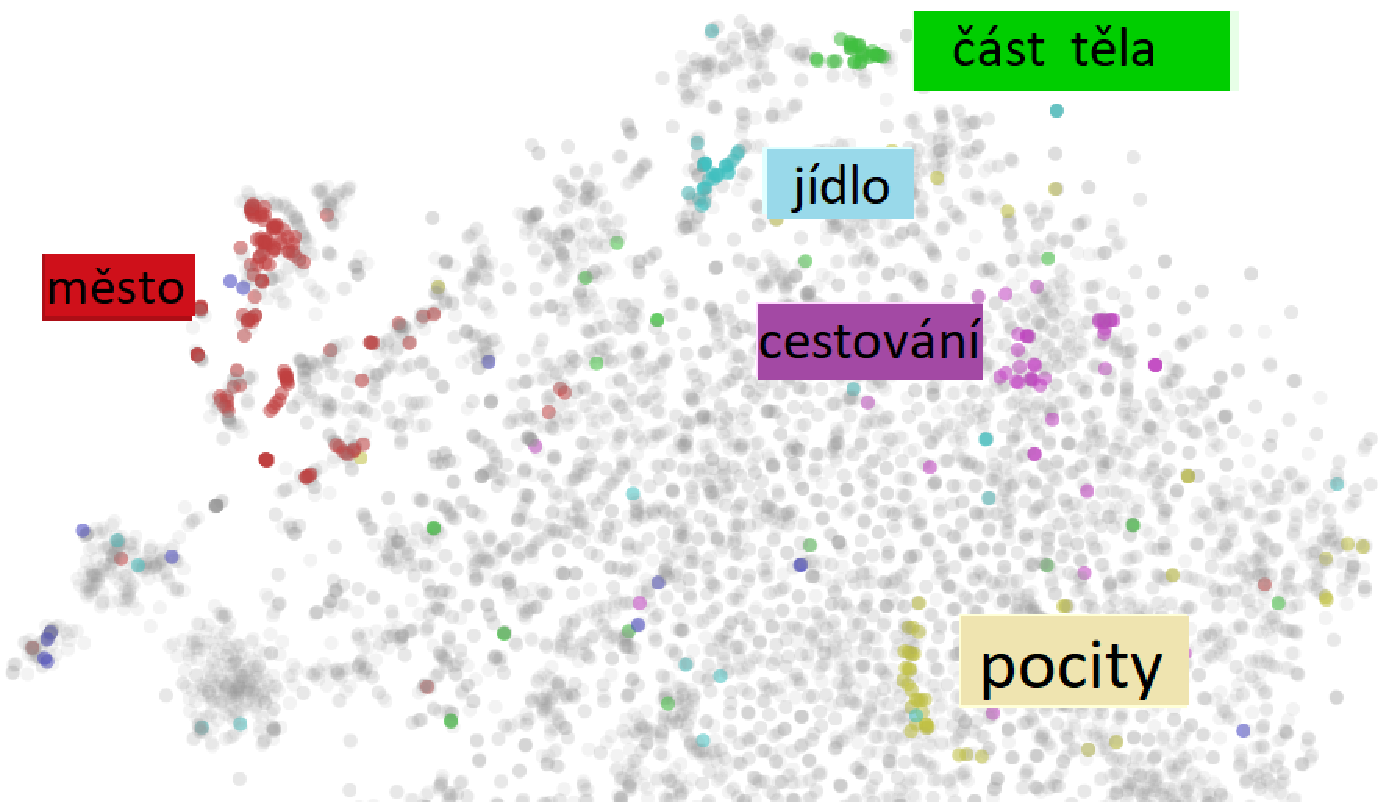
\includegraphics{obrazky/word_represent.pdf}}
	\caption{Část vektorového prostoru znázorňující reprezentace slov, která spojuje nějaké téma. Převzato z \cite{online:word_embedds}.}
	\label{word_embeddings}
\end{figure}
%=========================================================================

\subsection{Word2vec}

Word2vec je technika prezentována v~článku \cite{mikolov2013embeddings}, schopná naučit se vektorové reprezentace pomocí prediktivního modelu neuronové sítě. Základním konceptem dvou přístupů, které se pro trénink modelu používají, je predikce slov na základě slov sousedních v~tzv. kontextovém okně, které se postupně posouvá. Dostáváme tak pro každé slovo pravděpodobnost, se kterou se může vyskytovat v~blízkosti slova cílového.\par
První model používaný pro trénink word2vec vektorů se anglicky označuje jako Continuous Bag of Words, neboli CBOW. Skrytá projekční vrstva neuronové sítě se trénuje hádáním chybějícího slova v~kontextu již známých sousedních slov kontextového okna.\par
Druhá metoda funguje na opačném principu a~nazývá se Continuous Skip-gram Model. Na základě současného slova se model snaží předpovědět slova v~určité vzdálenosti před i~po současném slově, v~závislosti na velikosti kontextového okna. Tato metoda se z~článku~\cite{mikolov2013embeddings} jeví jako o~něco úspěšnější.\par
Na obrázku \ref{cbow_and_skipgram} je vidět rozdíl v~tom, jak projekční vrstva transformuje vstup na výstup v~případě obou architektur.

\begin{figure}[hbt]
	\centering
	\scalebox{0.5}{
	    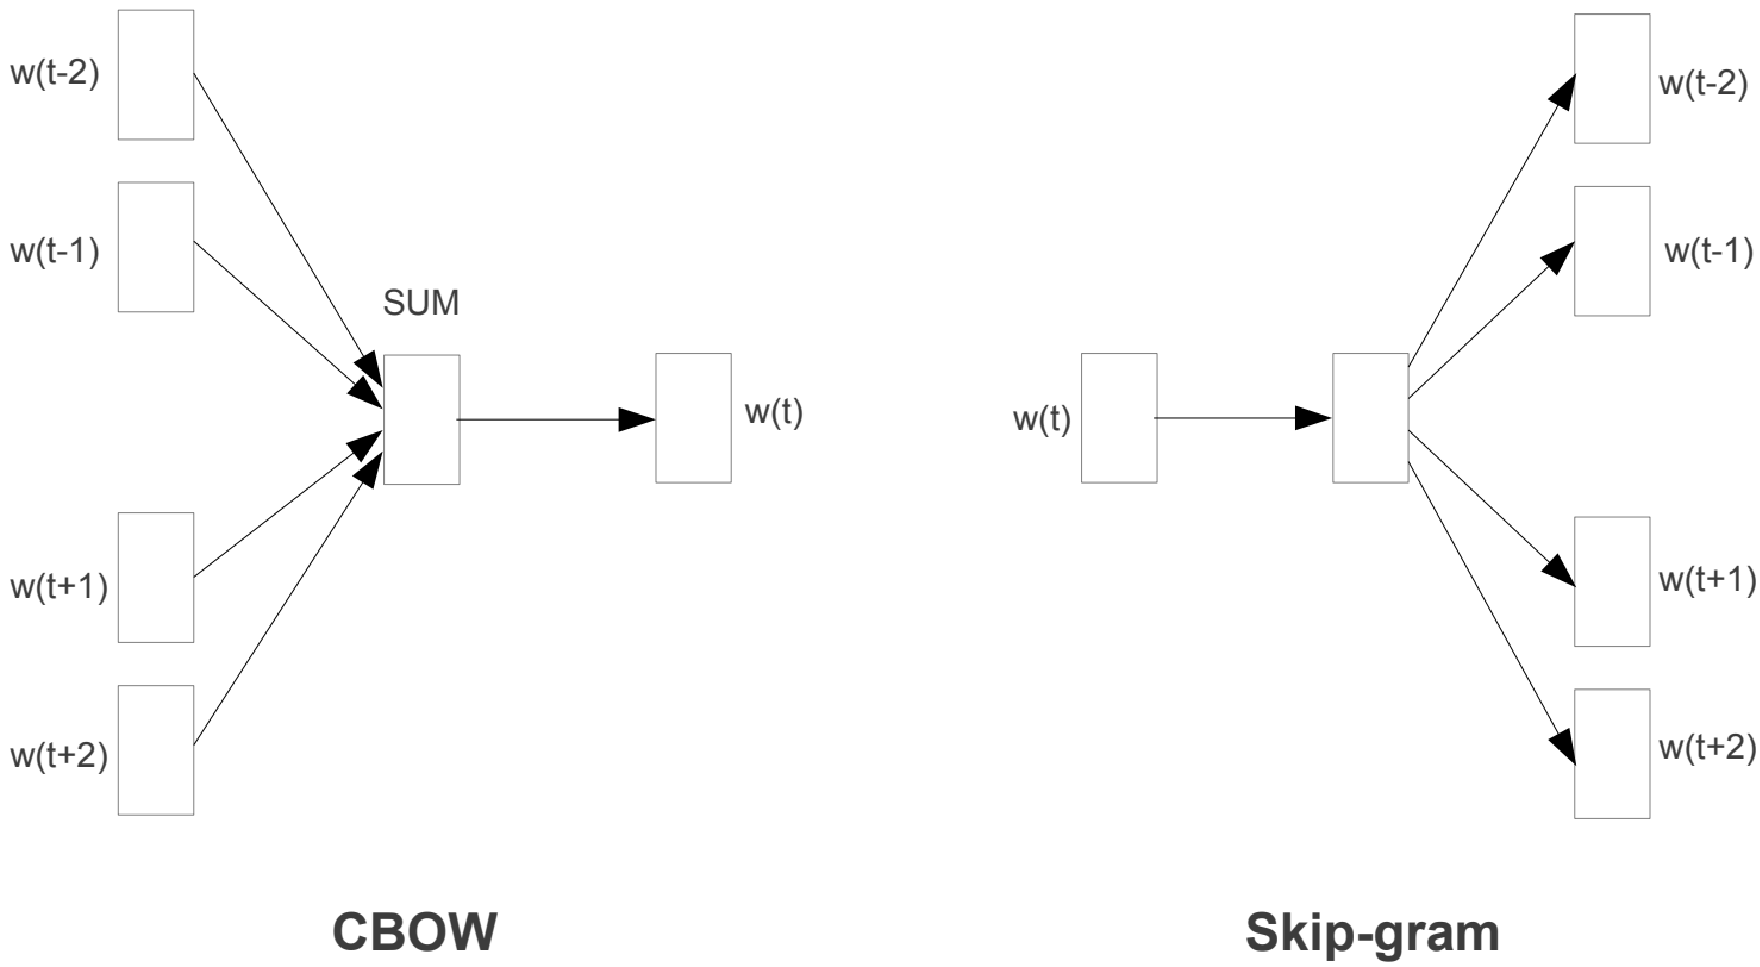
\includegraphics{obrazky/cbow_skipgram.pdf}}
	\caption{Obrázek architektury CBOW, předpovídající slovo na základě kontextu, a Skip-gram, předpovídající kontext na základě slova. Kontextové okno je znázorněno jako $w(t-2)$ až $(t+2)$. Převzato z \cite{mikolov2013embeddings}.}
	\label{cbow_and_skipgram}
\end{figure}

%=========================================================================

\subsection{GloVe}

GloVe, neboli Global Vectors for Word Representation, je technika představená v~článku \cite{GloVe}. Výsledkem je vektorový prostor o~pevně dané dimenzi, stejně jako u~word2vec. Liší se však způsobem získání daných reprezentací.\par Zatímco word2vec je prediktivní model, GloVe je spíše modelem statistickým. Klade tedy důraz hlavně na počet výskytů slov a~počet jejich výskytů v~podobných kontextech. Dostaneme tedy nějakou matici společných výskytů slov v~korpusu.\par
Hlavní výhodou tohoto modelu je, že se nesoustředí pouze na slova v~těsném kontextu, jak už slovo \emph{Global}, ukryté v~GloVe, napovídá. Reprezentace je tedy schopna zachytit sémantické souvislosti v~širším kontextu. Nicméně základní idea není konceptu word2vec příliš vzdálena.

%=========================================================================

\subsection{Wordpiece embeddings}
\label{wordpiece_embb}
Wordpiece je prediktivní technika, představená v článku \cite{wordpiece}, původně určená pro strojový překlad, která je také používána modely popsanými v~podkapitole \ref{bert_albert}.\par
Hlavním záměrem přístupu je lépe se vypořádat s~ojedinělými slovy tak, že jsou slova rozdělena do již známých \emph{podslov}. Nabízí tím kompromis mezi \emph{word embeddings} pro celá slova a~tzv. \emph{character embeddings} pro jednotlivé znaky.\par
Slovník je nejprve naplněn všemi znaky v~textu a na tomto slovníku je trénován jazykový model. Z~výsledného slovníku modelu je poté sestaven slovník nových kombinací jednotlivých znaků tak, aby se zlepšila úspěšnost na trénovací datové sadě. Postup se opakuje, dokud nenarazíme na limit minimální velikosti slovníku, nebo je rozdíl mezi úspěšností jednotlivých iterací modelu příliš malý.

%=========================================================================
\section{Tokenizace a~předzpracování}
\label{preprocessing}
Prvotní vyznačení základní struktury a předzpracování textu je důležitou součástí oblasti zpracování přirozeného jazyka. Cílem je transformovat vstupní text do podoby, který je pro automatické zpracování vhodnější. \par
První část této podkapitoly navazuje na část \ref{reprezentace_slov} o~reprezentaci jednotlivých slov textu. Zabývá se postupem rozdělení textu na tzv. \emph{tokeny}, které mohou být později převedeny na jejich vektorovou reprezentaci. Druhá část je potom věnována postupům pro zpracování a normalizaci textu pro optimální využití hodnotících funkcí. Jak se ukazuje, statistické metody, využívané těmito algoritmy, fungují lépe, pokud jsou z~textu odstraněna slova nesoucí pouze malou informaci. \par
Poznamenejme na tomto místě tak, že jednotlivé nástroje pro efektivní zpracování textu, přímo použité v~této práci, jsou uvedeny v~podkapitole \ref{pouzite_nastroje}.

\subsection{Tokenizace vstupního textu}
\textbf{Tokenizace} je převod textu z posloupnosti jednotlivých znaků na posloupnost jednotlivých tokenů. Například rozdělení textu \uv{Adam šel po škole domů.} na posloupnost tokenů:
\begin{center}
    \_Adam $+$ \_šel $+$ \_po $+$ \_škole $+$ \_domů $+$ \_.
\end{center}
Primitivním přístupem může být rozdělení textu pomocí bílých znaků a~interpunkčních znamének, které však nebere ohled např. na tečky ve zkratkách a špatně se vypořádává se složeninami. Získané tokeny je pak také potřeba normalizovat pro následný převod na word embeddings.\par
V~přístupu uvedeném v~podkapitole \ref{wordpiece_embb} jsou slova dělena na tokeny podle toho, která podslova v~daném textu jsou slovníku známa. Anglická věta \uv{I~like playing.} by tedy byla převedena na následující tokeny:
\begin{center}
    \_I $+$ \_like $+$ \_play $+$ \_ing $+$ \_.
\end{center}
Na uvedeném případě je stěžejní hlavně převedení posloupnosti znaků \uv{playing} na dva podřetězce (tokeny) \emph{play} a~\emph{ing}. V podkapitole \ref{bert_albert} budou ještě uvedeny podobné příklady. 

\subsection{Normalizace délky textu a~rozdělení do vět}
V~kontextu práce je normalizací délky textu myšlena jakási standardní maximální délka dokumentu, ze kterého je později provedena extrakce správné odpovědi. Tento přístup je užitečný z několika důvodů.\par
Algoritmy pro řazení dokumentů dle relevance sice berou na relativní délku textů ohled, nicméně některé články, např. \cite{bm25_too_long}, naznačují, že příliš dlouhé dokumenty mohou být systematicky znevýhodňovány. Citovaný článek sice představuje úpravu klasického algoritmu pro minimalizaci tohoto problému, jsou v něm ale uvedeny i další důvody, proč je vhodné délku jednotlivých odstavců normalizovat.\par
Model pro vyznačení správné odpovědi v~textu je trénován na datové sadě, která příliš dlouhé dokumenty nebere v~úvahu\footnote{Pro každou otázku je jen jeden odstavec kontextu, ne celý článek z~Wikipedie.} a~jak je naznačeno v~článku \cite{QA_long_multiple_span}, není na dlouhých dokumentech příliš úspěšný.\par
Dalším důvodem je snaha nepřekládat pro účel vyznačení správné odpovědi (experimenty s modelem ALBERT v \ref{albert_eval}) příliš dlouhé úseky textu.\footnote{Hlavně kvůli určitým omezením dostupných nástrojů pro překlad.}

\paragraph{Proč rozdělit text do vět?}
Předpokládejme, že je text již rozdělen do jednotlivých odstavců. Pro každý odstavec je kontrolována jeho délka, jestli nepřesahuje délku maximální. Pokud je maximální délka odstavce překročena, může být sice rozdělen jednoduše na poloviny, na třetiny a~tak dále podle potřeby, bude tím ale ztracena velká část kontextu při rozdělení některých vět.\par
Pro takový případ je vhodné vědět, kde jednotlivé věty začínají a~končí, aby bylo možné jednotlivé odstavce případně smysluplně rozdělit. Vhodné je také zařídit, aby se jednotlivé rozdělené \uv{pododstavce} částečně překrývaly a~obsahovaly třeba 3 poslední věty odstavce předchozího -- pro maximální zachování původního kontextu.

\subsection{Převod na malá písmena}
\label{prevod_na_mala}
Převod na malá písmena je sice velmi jednoduchý, ale přesto užitečný krok. Při psaní otázky např. na virtuální klávesnici mobilního telefonu je velmi pravděpodobně, že uživatel napíše \uv{cd-rom} místo \uv{CD-ROM}, ale je nutné, aby byly nalezeny dokumenty obsahující obě varianty. Stejně tak může dojít k~nestandardnímu užití malých/velkých písmen v~některém z~dokumentů.\par
Pro některé případy může převod na malá písmeny znamenat ztrátu části kontextu. Například \emph{Malá Strana} X \emph{malá strana}, kde velké písmeno indikuje vlastní jméno (městskou část). Vhodné je to tedy pouze v~některých případech.

\subsection{Odstranění stop slov}
\label{stopwords}
Ve zpracování přirozeného jazyka jsou \emph{stop slova} typicky souborem nejčastěji používaných slov v~daném jazyce \cite{information_retrieval}. Většinou jsou odstraňována, protože kvůli jejich vysokému výskytu nesou menší informační hodnotu a~jejich odstranění vede k~lepší funkci vyhledávacích algoritmů a hodnotících funkcí \cite{bm25_improvements}.\par
Nejužívanější slova daného jazyka (například češtiny) je možno najít ve frekvenčních seznamech. Získaný seznam je vhodné kriticky zhodnotit a~vyčlenit z~něj některá slova, která by pro vyhledávání mohla mít kritický význam.\footnote{Příklad: \uv{první}, \uv{země}, \uv{člověk} \dots} Většinou je zanedbatelná  většina funkčních slov -- spojek, předložek či zájmen. Typickými příklady stop slov pro češtinu jsou: být, a, se, v, že \dots

\subsection{Získání lemmat}
\textbf{Lemmatizace} je druh zpracování textu, při kterém je pro každé slovo nalezen základní tvar, tzv. \emph{lemma}.\footnote{Podobným postupem je \emph{stematizace}, která ale algoritmicky pouze odstraní koncovky a~předpony pro nalezení slovního kmene \cite{information_retrieval}.}
\begin{center}
    ulicí běžely děti $\longrightarrow$ ulice běžet dítě\\
    ostrovy Středozemního moře $\longrightarrow$ ostrov Středozemní moře
\end{center}
Pro získání lemmat se používají speciální nástroje pro zpracování přirozeného jazyka. \emph{Lemma\-tizátory} mohou poskytovat také některé doplňkové informace o~mluvnických kategoriích jako rod, pád nebo slovní druh. Hlavním úskalím lemmatizátorů je mnohoznačnost jazyků jako je čeština, kdy může být více základních tvarů daného slova dle kontextu \cite{information_retrieval}. Potom přichází na řadu zjednoznačňování lemmat na základě kontextu.\par
Využití lemmatizace je různé, ale v~případě této práce je podobné, jako účel postupu uvedeného v~podkapitole \ref{prevod_na_mala} (převod na malá písmena). Lemmatizace je také užitečným nástrojem při odstranění stop slov. Mohou být odstraněny například všechny tvary slovesa \uv{být}, zatímco seznam stop slov může obsahovat pouze jeho základní tvar.


%=========================================================================
%===============================================================================

\chapter{Strojové učení pro extrakci odpovědi}
\label{language_comprehension}

Rozmach strojového učení umožnil obrovský pokrok v~oblastech NLP, jako je strojový překlad, rozpoznání entit, generování textu nebo odpovídání na otázky. Proto na tomto přístupu staví všechny nejmodernější metody a~tímto směrem se také ubírá aktuální výzkum.\par
Účelem této kapitoly je vysvětlit čtenáři, jak fungují neuronové sítě a~jakým způsobem dokáže počítač porozumět textu a~naučit se vyznačit v~textu odpověď na danou otázku.\par
Nejprve jsou ve zkratce vysvětleny principy fungování a~učení neuronových sítí. Poté jsou rozebrány nejznámější architektury neuronových sítí, používané pro vypořádání se s~úkoly na poli zpracování přirozeného jazyka, a popsány jsou také nejmodernější modely, které na nich staví a jsou vhodné pro extrakci odpovědi z textu.
\bigskip

%=========================================================================
\section{Neuronové sítě}
\label{neuronove_site}
V~této podkapitole je vysvětlen princip fungování neuronových sítí. Informace byly převzaty z~článku \cite{neural_nets} a~z~prezentací stanfordského kurzu NLP \cite{stanford:nlp}.\par
Neuronovou síť si můžeme zjednodušeně představit jako velkou funkci s~obrovským množstvím parametrů, která přetváří vstupy na výstupy. V~průběhu tréninku neuronové sítě se postupně všechny parametry optimalizují tak, aby síť přetvářela vstupy na výstupy co nejlépe.\par
Základem jsou tři jednoduché vrstvy (obrázek \ref{three_layers}). Vstupní, skrytá (zde probíhá proces přetváření vstupů) a~výstupní, kde se přetvořený vstup objeví. Skrytá vrstva se navíc běžně skládá z~mnoha dalších vrstev.\par
Každá z~těchto vrstev, ať už je vstupní, výstupní nebo skrytá, se skládá z~neuronů. Každý neuron v~určité vrstvě je propojen s~každým neuronem vrstvy další, a~tak je propojena celá síť.

\begin{figure}[hbt]
	\centering
	\scalebox{0.50}{
	    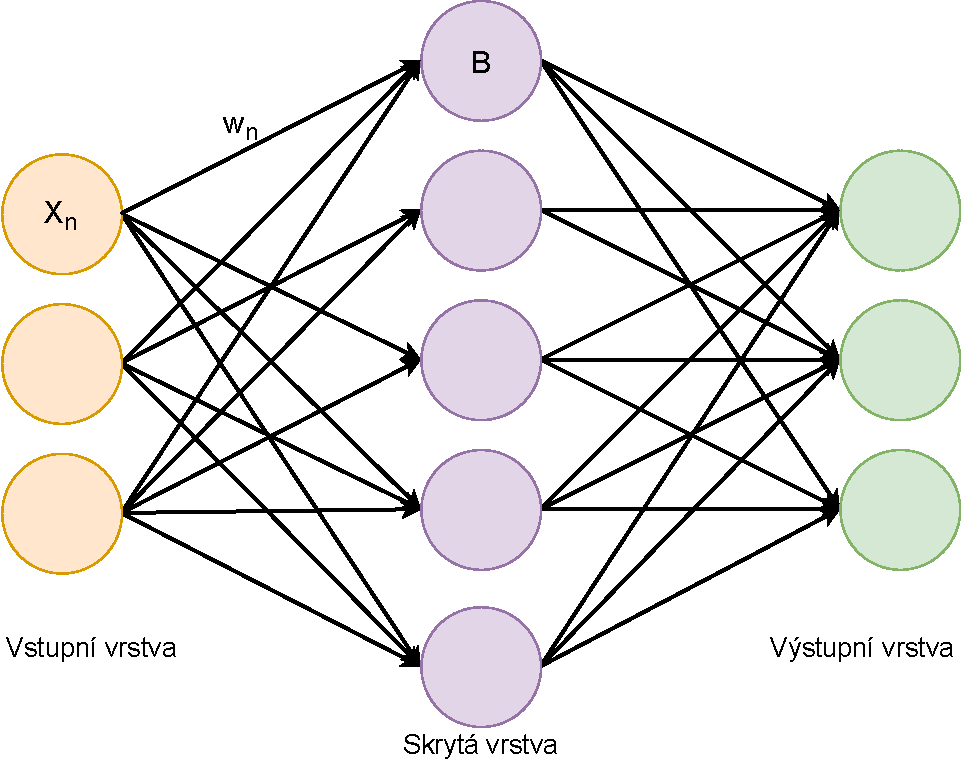
\includegraphics{obrazky/neural_net.pdf}}
	\caption{Schéma neuronové sítě s jedinou skrytou vrstvou. Znázorněn je také jeden vstup neuronu $B$ z předchozí vrstvy $x_n$ a váha jeho propojení $w_n$.}
	\label{three_layers}
\end{figure}

\subsection{Umělý neuron a~aktivační funkce}
Umělý neuron je primitivní jednotka, inspirovaná neuronem skutečným. Ten má tělo, do kterého přichází krátkými výběžky, tzv. \emph{dendrity}, elektrické signály z~ostatním neuronů. Z~těla neuronu pak vychází jediný dlouhý výběžek, tzv. \emph{axon}. Neuron se tedy na základě signálů, které do něj přichází dendrity, rozhodne (na základě nějaké minimální hranice přijatého signálu), zda bude, nebo nebude vysílat signál dál \cite{wiki:neuron}.\par
Funkce umělého neuronu je analogická. Jak už bylo popsáno v~úvodu podkapitoly~\ref{neuronove_site}, každý neuron je propojen s~každým neuronem vrstvy předcházející i vrstvy další. Na rozdíl od skutečného neuronu má tedy více \uv{axonů}, kterými je propojen s~další vrstvou.\par
Každé propojení mezi dvěma neurony má svoji váhu \emph{w}, která ovlivňuje důležitost daného vstupu do neuronu. Každý neuron má také svůj práh \emph{B} a~aktivační funkci. Výstupem $y$ neuronu $i$ je tedy vážená suma vstupů do neuronu s~přičteným prahem a~aplikovanou aktivační funkcí, neboli 
\begin{equation}
y_i = F({\sum_{k=1}^n ({x_n}w_n)} + B_i)
\end{equation}
kde $x_n$ je neuron předcházející vrstvy, $w_n$ je váha jeho propojení, $B_i$ je práh aktuálního neuronu $i$ a~$F$ je aktivační funkce. Znázornění vah propojení a~jednotlivých neuronů je vyznačeno na obrázku \ref{three_layers}.\par
Všechna propojení jednotlivých neuronů s~jejich prahy dávají dohromady parametry neuronové sítě, které jsou v~průběhu tréninku optimalizovány pro každý neuron zvlášť. Pro síť, jako je na obrázku \ref{three_layers}, je to třeba 30 jednotlivých vah propojení a~8 prahů jednotlivých neuronů (skryté a~výstupní vrstvy), tedy 38 parametrů v~relativně jednoduché síti.\par
\textbf{Aktivační (přenosová) funkce} rozhoduje, jestli bude daný neuron aktivován. Skutečný neuron má, zdá se, funkci skokovou. Umělé neurony však používají funkce s~postupnou aktivací. Běžné jsou tři základní varianty aktivačních funkcí: 

\begin{itemize}
    \item Sigmoidální
    \item Hyporbolické tangenty
    \item ReLU (Rectified Linear Unit)
\end{itemize}
\pagebreak

Funkce jsou znázorněny na obrázku \ref{aktivacni_funkce}. Vhodnost jejich použití záleží na kontextu. Výhodou sigmoidální funkce je normalizace výstupu do rozmezí $(0,1)$. Nejpoužívanější funkcí pro skrytou vrstvou je však funkce ReLU. Kvůli její charakteristice je aktivováno méně neuronů, což vede k~rychlejšímu tréninku a~konvergenci. Použití ReLU funkce je také výpočetně méně náročné \cite{medium:activation_function}.

\begin{figure}[hbt]
    \centering
	    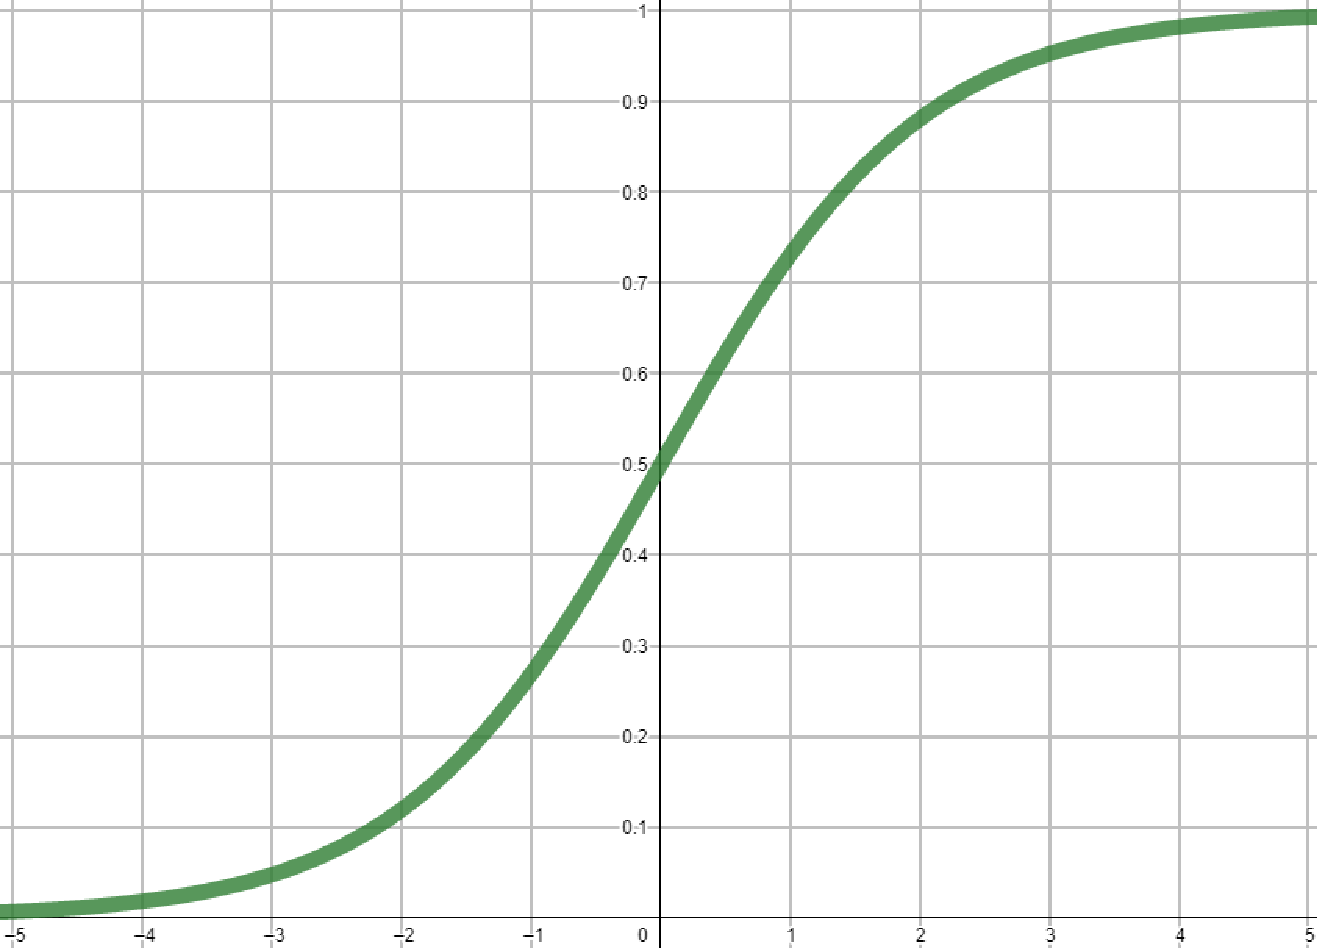
\includegraphics[width=0.33\linewidth, height=1.5in]{obrazky/sigmoid.pdf}\hfill
    	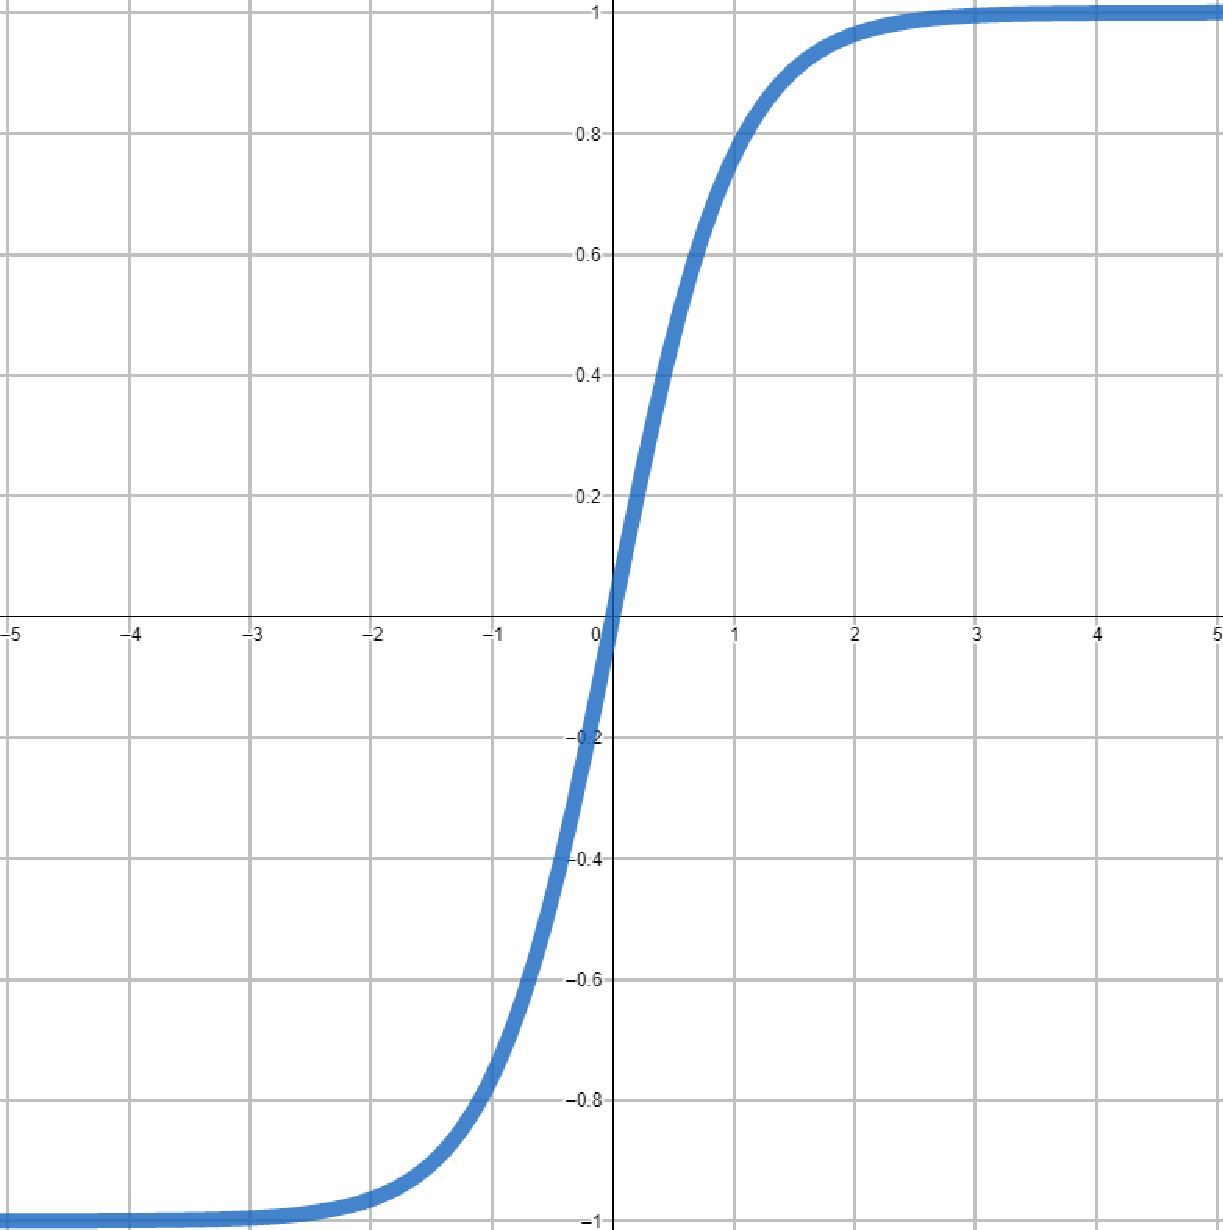
\includegraphics[width=0.33\linewidth, height=1.5in]{obrazky/tanh.pdf}\hfill
    	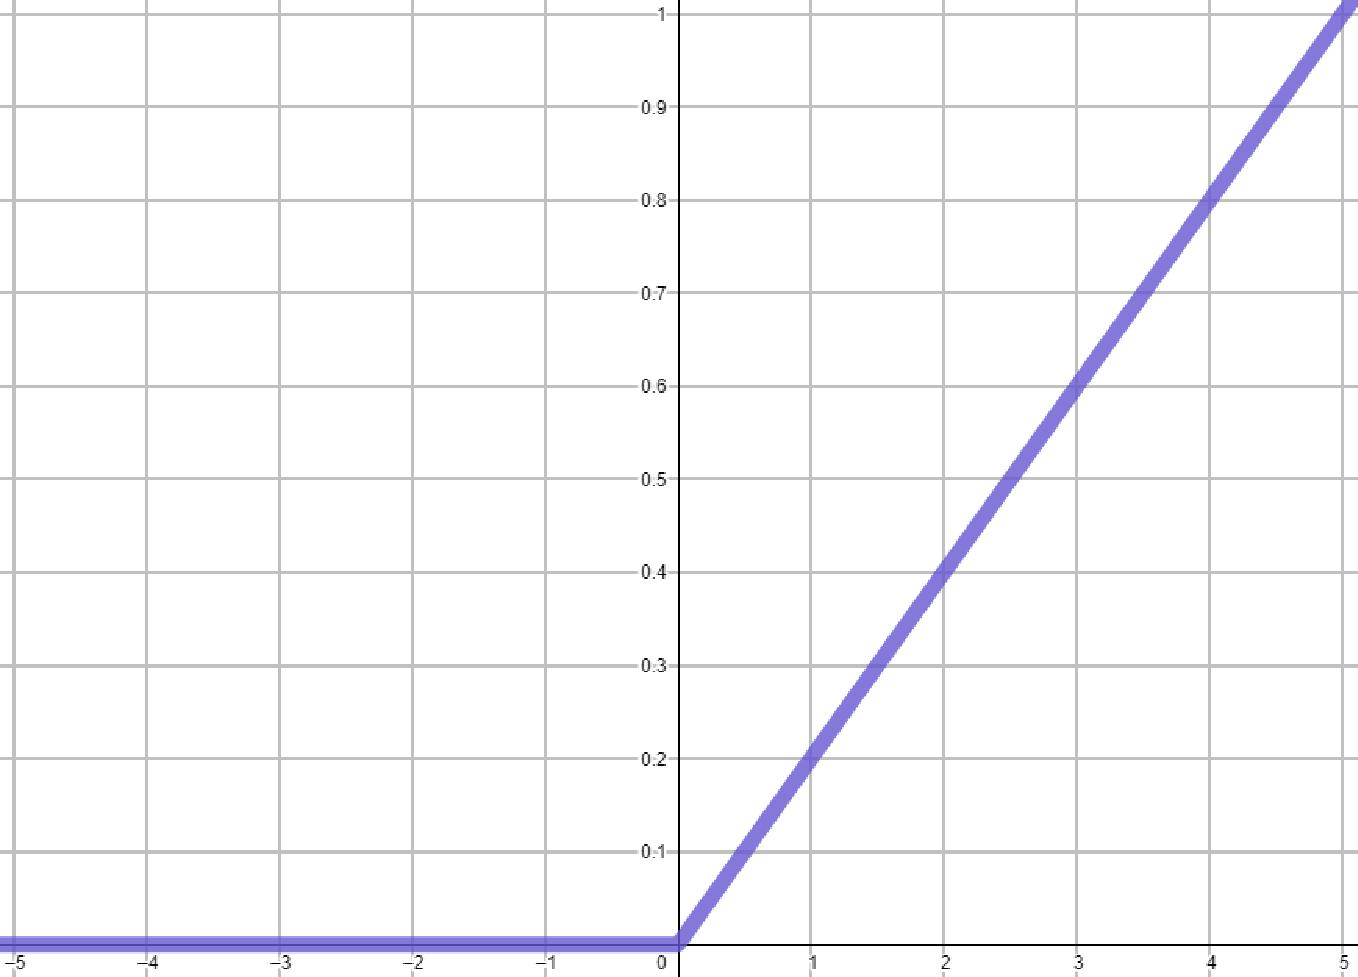
\includegraphics[width=0.33\linewidth, height=1.5in]{obrazky/relu.pdf}\hfill
	\caption{Jednotlivé aktivační funkce. Zleva: sigmoidální ($H(f)=\langle 0,1 \rangle$), hyperbolické tangenty (tanh $H(f)=\langle -1,1 \rangle$) a ReLU ($H(f)=\langle 0,\inf \rangle$).}
	\label{aktivacni_funkce}
\end{figure}


\subsection{Dopředná a~zpětná propagace}
Proces, kdy se opakovaně ze vstupů počítá výstup každého neuronu v~dané vrstvě, a~stejně tak pro každou následující vrstvu, se nazývá dopředná propagace. Hodnoty vstupní vrstvy se postupně přetvoří na hodnoty ve vrstvě výstupní a~může se určit, jak byla síť v dané iteraci úspěšná.\par
Pro určení úspěšnosti každé takové iterace neuronové sítě se používá nákladová funkce (anglicky \textit{cost function} pro jednu iteraci, \textit{loss function} pro průměr všech), která udává jediné číslo, charakterizující úspěšnost modelu. Nejznámější nákladovou funkcí je střední kvadratická chyba (anglicky \textit{Mean Squared Error} -- MSE). Cílem je hodnotu této nákladové funkce postupně minimalizovat.\par \medskip
Postup optimalizace jednotlivých parametrů neuronové sítě pro zajištění minimalizace nákladové funkce se nazývá \textbf{zpětná propagace}. Je to v~podstatě opačný průchod neuronovou sítí, který má za úkol zjistit, které neurony se největší mírou podílely na výsledné chybě. Snížením významu těchto neuronů můžeme dosáhnout lepší úspěšnosti celé sítě. Naopak můžeme zvýšit význam propojení s~neurony, které výstup ovlivnily pozitivně.\par
Základem tohoto výpočtu je, že chyba každého výstupního neuronu je vstupem parciální derivace vzhledem ke každému z~jeho vstupů. Zpětná propagace je opakována v každé iteraci a~parametry neuronové sítě jsou postupně optimalizovány \cite{neural_nets}.\par
Celý postup zpětné propagace je složitější a~pro intuitivní pochopení problematiky není klíčový, proto tu není podrobně rozebrán.\par
\medskip
Trénink neuronové sítě tedy probíhá následovně. Síti s~náhodně inicializovanými parametry je předložena část dat z~trénovací datové sady. Ty jsou pomocí dopředné propagace prostupem přes skryté vrstvy přetvořeny na výstupy, čímž jsou získány predikce neuronové sítě. Predikce jsou porovnány se správnými očekávanými hodnotami (tzv. \emph{ground truth}) a~nákladovou funkcí je vyjádřeno, jak byly predikce daleko od očekávaných. Pomocí zpětné propagace jsou postupně upraveny všechny parametry neuronové sítě.\par
Postup je opakován, dokud úbytek nákladové funkce mezi jednotlivými iteracemi nezačne dlouhodobě stagnovat, nebo dokud nedosáhneme požadovaného počtu epoch.\par
Při nesprávném tréninku neuronové sítě může dojít k~podtrénování (\textit{underfitting}), nebo přetrénování (\textit{overfitting}). Problémy při tréninku souvisí s~tzv. hyperparametry, mezi které patří počet skrytých vrstev, velikost modelu nebo parametrem \emph{learning rate}\footnote{Parametr \emph{learning rate} určuje velikost kroku při každé iteraci zpětné propagace, tedy úpravě parametrů neuronové sítě.}. Pomoci může také množství trénovacích dat nebo počet trénovacích epoch.

%=========================================================================
\section{Nejlepší architektury pro porozumění textu}
V~této podkapitole jsou popsány dvě nejznámější a~nejpoužívanější architektury pro zpracování přirozeného jazyka. Rozšiřují koncepty prezentované v~podkapitole \ref{neuronove_site} a~snaží se překonat problémy, které tradiční model neuronové sítě v souvislosti s porozuměním textu nese.\par

\subsection{Long short-term memory}
\label{lstm}
Informace v~této podkapitole byly čerpány z~prvotní práce \cite{LSTM}, která architekturu představuje,  a~článku \cite{understandingLSTM}, poskytujícího vysvětlení některých konceptů.\par
LSTM, neboli Long Short-term Memory, je speciální druh \emph{rekurentní} neuronové sítě, který se částečně vypořádává s~problémem ztráty kontextu v~delším úseku textu. Jednoduše řečeno, při učení neuronové sítě by bylo užitečné, aby pochopení současné věty dokázala ovlivnit i věta předcházející.\par

\begin{figure}[hbt]
    \centering
	\scalebox{0.9}{
	    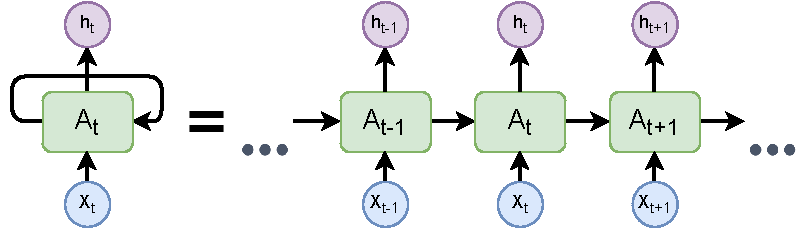
\includegraphics{obrazky/rnn.pdf}
	}
	\caption{Schéma rekurentní neuronové sítě -- inspirováno obrázkem z \cite{understandingLSTM}. $X_t$ je vstupem neuronové sítě $A_t$ v čase $t$ a výstupem $h_t$.}
	\label{RNN}
\end{figure}

Nejprve vysvětleme princip \textbf{rekurentní neuronové sítě} (dále RNN -- \textit{Recurrent Neural Network}).
Hlavním cílem této architektury je vypořádat se se zpracováním sekvenčních dat, jako je text. Oproti například rozpoznávání vzorů v~obrázcích není možné pohlížet na každé slovo v~textu zvlášť. Slovo/slova předcházející by měla ovlivnit slovo současné. Stejně tak mohou následující slova ovlivnit význam slova současného (obousměrné rekurentní sítě).\par
Schéma jednoduché RNN je vidět na obrázku \ref{RNN}. Zjednodušeně je to tedy více jednoduchých neuronových sítí propojených za sebe. Vstupem každé sítě $A_t$ v čase $t$ je výstup sítě $A_{t-1}$. Výstup $h_t$ je pak vstupem sítě $A_{t+1}$.\par
Analogicky funguje obousměrná RNN, které je propojena i v~opačném směru. Vstup je zpracováván od konce a~pro současné slovo je tedy brán v~úvahu i kontext slova následujícího, jak je vidět na obrázku \ref{bidirRNN}.\par

\begin{figure}[hbt]
    \centering
	\scalebox{0.9}{
	    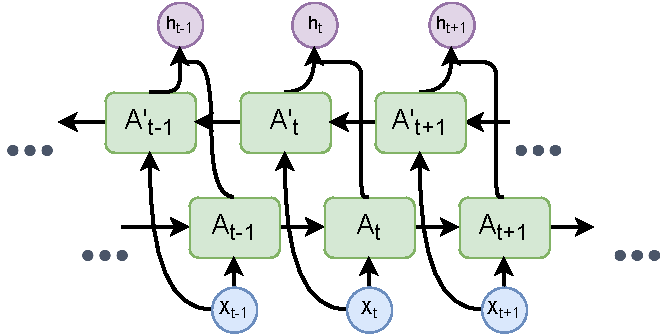
\includegraphics{obrazky/bidir_rnn.pdf}
	}
	\caption{Schéma obousměrné rekurentní neuronové sítě.}
	\label{bidirRNN}
\end{figure}

\pagebreak\textbf{LSTM} (Long Short-term Memory) představuje vylepšení standardní RNN. Mějme model, který má za úkol předpovědět následující slovo ve větě. Pokud se kontext potřebný pro predikci nachází v~těsné blízkosti předpovídaného slova (př.: \uv{vychlazené mléko z~\emph{lednice}}), je i běžná RNN schopna souvislost zachytit. Pro příklad, kdy je kontext \uv{dále v~minulosti} (př.:\uv{Učím se od 6 let anglicky \dots Vzhledem k~těmto okolnostem plynule ovládám \emph{angličtinu}}), nemusí být RNN schopna naučit se tuto souvislost mezi kontextem a~hledaným slovem.\par \smallskip
LSTM je  na rozdíl od klasické RNN navržena tak, aby byla schopna pamatovat si dlouhodobé souvislosti v~textu při sekvenčním zpracování. Řeší tím tzv. \emph{problém mizejícího gradientu}.\par
Model má stejnou opakující se strukturu jako RNN, rozdíl je však v~komplexnosti opakující se jednotky (či buňky). Struktura naznačená na obrázku \ref{lstm_cell} je poměrně složitá a~jejím hlavním komponentem jsou tzv. \emph{brány}. 

\begin{figure}[hbt]
    \centering
	\scalebox{1}{
	    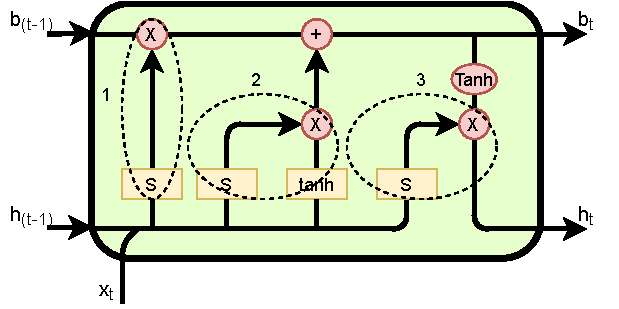
\includegraphics{obrazky/lstm_cell.pdf}
	}
	\caption{Schéma LSTM buňky, převzato z článku \cite{understandingLSTM}. $b_t$ je vnitřní stav buňky, $b_{(t-1)}$ předcházející buňky, $h_t$ výstup buňky, $h_{(t-1)}$ výstup předcházející. $x_t$ je vstup současné buňky. \uv{1} je \emph{zapomínací}, \uv{2} \emph{vstupní} a \uv{3} \emph{výstupní} brána.}
	\label{lstm_cell}
\end{figure}

Brány jsou v~LSTM buňce celkem tři. Každá je složena z~vrstvy neuronové sítě se sigmoidální funkcí (\uv{S} v \ref{lstm_cell}) a~násobícího (\uv{$\times$} v \ref{lstm_cell}) operátoru. Brána je komponentem určujícím, kolik informace je možno propustit. Brány jsou popsány zleva doprava.\par
První, tzv. zapomínací brána určuje, kolik vstupní informace je zahozeno\footnote{Výstupem je číslo v~rozmezí (0,1), kde 0 znamená \uv{všechno zahodit} a~1 znamená \uv{všechno propustit}.}. Druhá, tzv. vstupní brána, určí, které hodnoty skrytého stavu buňky budou aktualizovány a~vrstva s~funkcí \emph{tanh} (\uv{tanh} v \ref{lstm_cell}) rozhodne o~nových kandidátních hodnotách, které po kombinaci s~výstupem sigmoidální vrstvy vytvoří nový skrytý stav buňky. Poslední brána je výstupní, spojuje informaci z~brány zapomínací s~vnitřním stavem buňky, a~vytváří tím tedy výstup dané buňky.\par
Jednotlivé LSTM buňky jsou za sebou sekvenčně propojeny stejně jako RNN. Při použití dvou LSTM sítí, kdy druhá je propojena v~opačném směru, získáme obousměrnou LSTM síť. Výstupy obou sítí jsou poté pro získání výstupu zřetězeny.

\subsection{Transformers}
\label{transformers}
Informace v~této podkapitole byly převzaty z~prvotní práce \emph{Attention Is All You Need} \cite{Transformers}, dále z \cite{attention_mechanism} a~článku \cite{Transformers-explained}. Text popisuje  architekturu Transformers, používanou pro zpracování přirozeného jazyka. Také se věnuje mechanismu pozornosti (\emph{attention}).\par
Přístup použitý tímto modelem se dokázal oprostit od rekurentních modelů jako LSTM a velmi rychle se etabloval jako  nejlepší současná architektura na poli zpracování přirozeného jazyka. Sítě typu transformer nepoužívají sekvenční zpracování slov, ale zpracování paralelní. Nejdůležitější myšlenkou je  mechanismus pozornosti, představený článkem \cite{attention_mechanism}, původně pro strojový překlad. Ten se dále rozvíjí a jeho varianty pronikají i do dalších odvětví aplikací strojového učení. Stručně je popsán v následujích odstavcích.\par \medskip

Mechanismus pozornosti vezme vektory dvou vět přirozeného jazyka naráz a~sestaví z~nich matice \emph{key(\textbf{K})-value(\textbf{V})} a~\emph{query(\textbf{Q})}, obsahující v řádcích vektory pro každé vstupní slovo. Ty vzniknou vynásobením vstupní matice word embedding  speciální váhovou maticí, jejíž parametry jsou trénovány. Na matice jsou poté aplikovány následující operace pro získání výstupu pozornosti (rovnice \ref{attention_dot_product}).

\begin{equation}
    \label{attention_dot_product}
    softmax(\frac{Q \times K}{k})\times V
\end{equation}

V rovnici \ref{attention_dot_product} je $k$ podle \cite{Transformers} konstanta 8 (mohly by být stanoveny i jiné hodnoty) a~softmax funkce je použita pro normalizaci výstupu do rozmezí (0,1).\par
Vektory pro všechna vstupní slova, respektive vstupní matice K, V~a Q, mohou být ze stejné věty. Pro tuto variantu mechanismu se používá termín \textbf{self-attention}.\par 
Jednoznačnou výhodou mechanismu pozornosti je, že je schopen podívat se na celý kontext současně (na rozdíl od RNN, která prochází vstup sekvenčně) a~vyznačit v~něm důležité pasáže. Tímto se zbavuje problému mizejícího gradientu.\par\medskip

\textbf{Transformer} enkodér\footnote{Enkodér je část modelu, která vytvoří z~vektorů jednotlivých slov na vstupu vektor celého vstupního textu, reprezentující jeho význam. V původním článku \cite{Transformers} je představen model pro \emph{sequence to sequence} model vhodný pro překlad, který obsahuje i dekodér pro generování textu.} je model, jehož architektura je kombinací dopředné neuronové sítě a~mechanismu pozornosti. Jak už bylo popsáno, jeho hlavní výhodou je vlastnost zpracovávat vstupní slova paralelně, a~tím se naučit i vztahy mezi slovy na dlouhé vzdálenosti v~textu.\par

\begin{figure}[hbt]
    \centering
	\scalebox{1}{
	    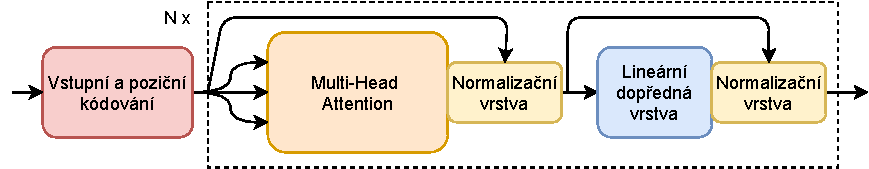
\includegraphics{obrazky/transformer_encoder.pdf}
	}
	\caption{Schéma architektury transformer enkodéru převzaté z článku \cite{Transformers}. V článku je uvedeno $N=6$ pro počet identických vrstev enkodéru. }
	\label{transformer_encoder}
\end{figure}

Na obrázku \ref{transformer_encoder} můžeme vidět zjednodušenou strukturu jednotky enkodéru. V~článku~\cite{Transformers} tvoří enkodér 6 takových bloků propojených za sebe.\par
Před vstupem do prvního bloku jsou jednotlivé tokeny vstupního textu převedeny na vektory (word embeddings), ke kterým je přidáno poziční kódování\footnote{identifikuje pořadí tokenu ve vstupním textu.}. Každý blok se pak skládá z~\uv{\emph{multi-head attention}} modulu a~plně propojené dopředné vrstvy. Obě části jsou následovány normalizační vrstvou.\par
Nejzajímavější částí bloku enkodéru je multi-head attention modul, který je dále rozkreslen na obrázku \ref{multihead}. Modul je sofistikovanou implementací self-attention mechanismu, popsaného dříve, který dokáže vyzdvihnout souvislost jednotlivých částí celého kontextu. 

\begin{figure}[hbt]
    \centering
	\scalebox{0.35}{
	    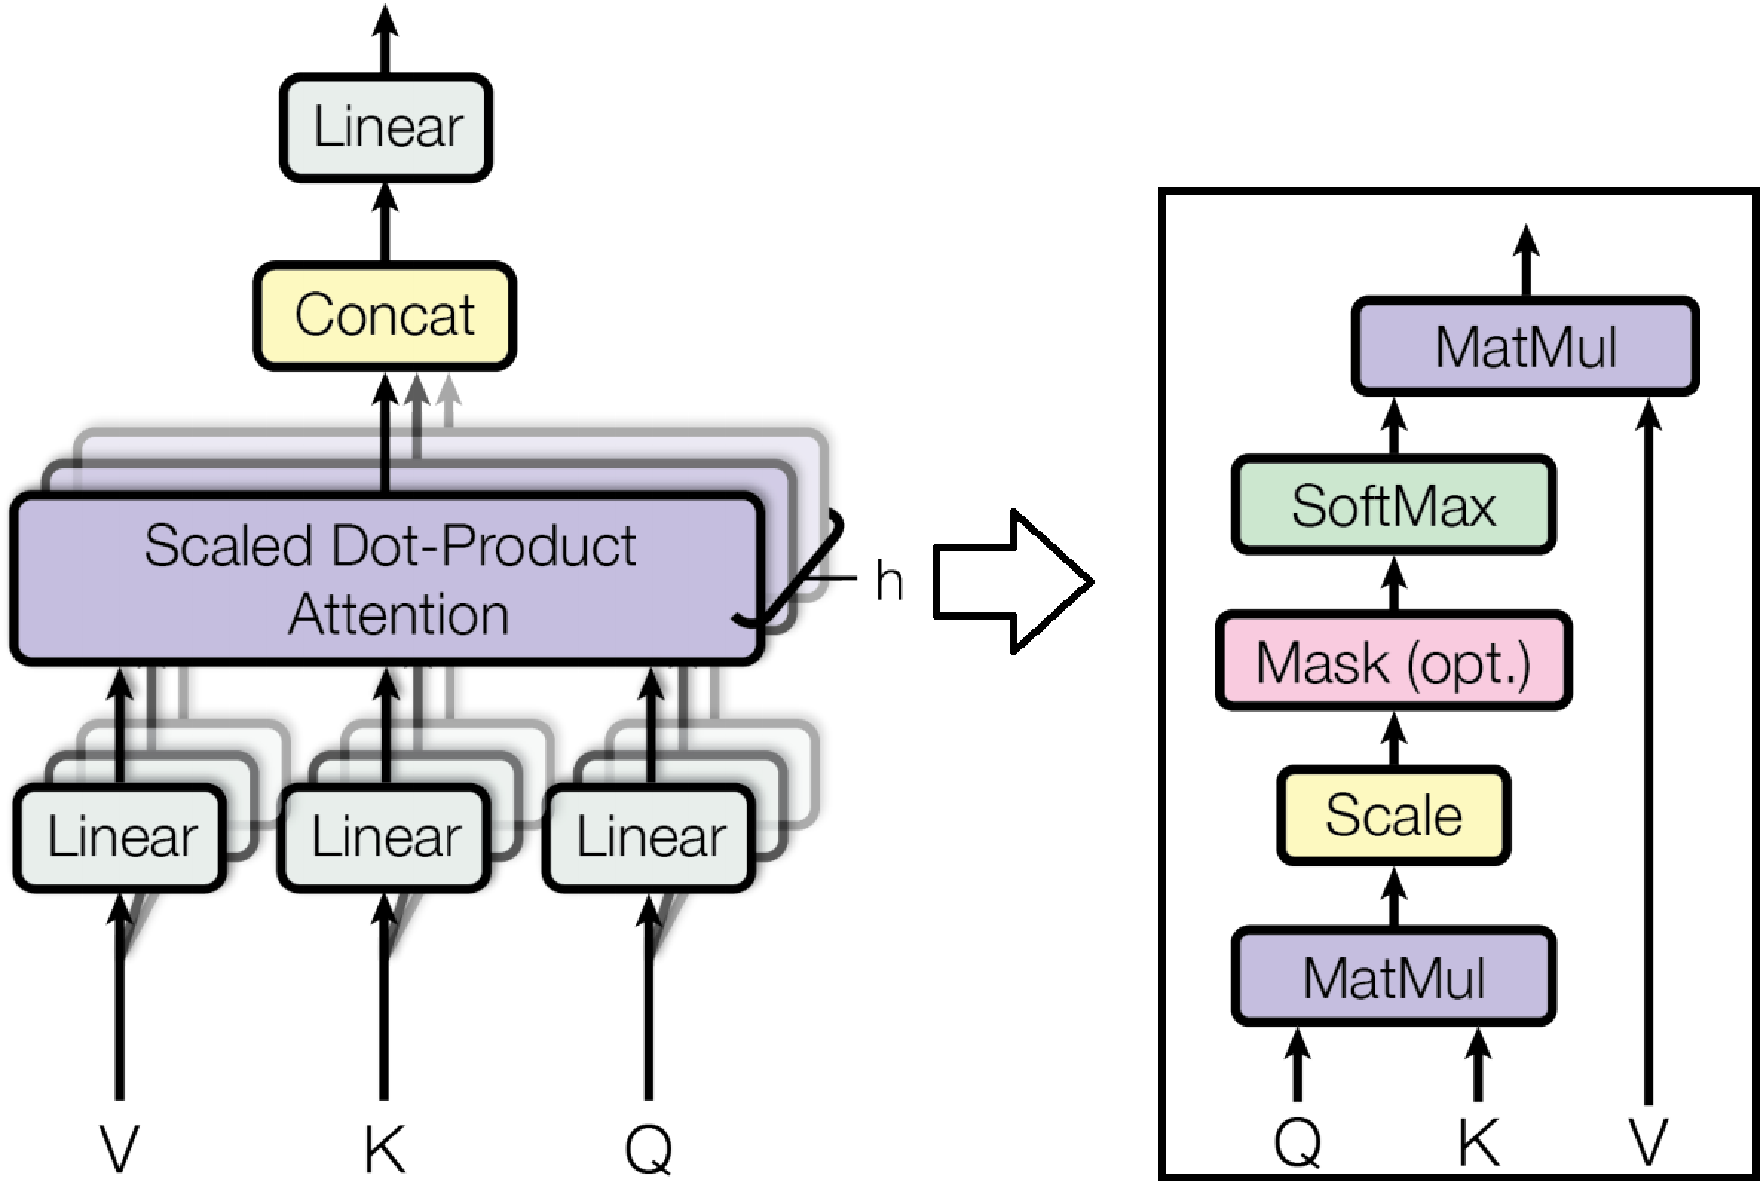
\includegraphics{obrazky/multihead_att.pdf}
	}
	\caption{Schéma \emph{Multi-Head} attention vlevo a \emph{Scaled Dot-Product} attention vpravo. \emph{Multi-head} attention je aplikováno paralelně v $h$ vrstvách (pro práci \cite{Transformers} $h=8$). Obrázky byly převzaty z článku \cite{Transformers}.}
	\label{multihead}
\end{figure}

Mechanismus na obrázku \ref{multihead} vpravo je popsán rovnicí \ref{attention_dot_product} a~je hlavním komponentem multi-head attention modulu, znázorněným v~\ref{multihead} vlevo.\par
Multi-head znamená, že do modulu vstupuje 8 (dle práce \cite{Transformers}) trojic V,K,Q. Každá matice trojice V,K,Q je transformována lineární vrstvou a~na celou trojici je potom aplikován \emph{scaled dot-product attention} (self-attention) mechanismus. Tento postup je aplikován na každou z~osmi trojic paralelně, pokaždé však s~jinými váhami lineární vrstvy.

%=========================================================================
\section{Předtrénované modely BERT a~ALBERT}
\label{bert_albert}

V~této podkapitole jsou představeny základní modely, založené na architektuře Transformer, která byla popsána výše. Informace v~této podkapitole  jsou převzaty z~původních článků \cite{BERT} a~\cite{ALBERT}.\par
Předtrénované modely, stavějící na této architektuře, určily nový standard pro nově vytvářené metody. Kromě jejich vysoké úspěšnosti je obrovskou výhodou také znovupoužitelnost předtrénovaných modelů. Modely je možno jednoduše dotrénovat (provést adaptaci po načtení modelu s~předtrénovanými parametry) pro celou řadu úkolů na poli NLP, jako je odpovídání na otázky, rozpoznání entit, klasifikace textu a~další.

\subsection{BERT}
BERT (\textit{Bidirectional Encoder Representation from Transformers}) je model pro reprezentaci přirozeného jazyka, představený v~roce 2018 prací \cite{BERT}. Jeho hlavním přínosem je aplikace obousměrného tréninku  architektury transformer. Ukazuje se, že model trénovaný v~obou směrech dokáže plně využít schopnost transformerů zpracovávat vstupní text naráz, nikoliv sekvenčně.\par\smallskip
Hlavním přínosem práce \cite{BERT} je způsob, kterým probíhá předtrénování na velkých textových korpusech. Trénink na úkolech, které nemusí přímo souviset s~cílovým použitím, dovolí modelu získat základní pochopení vlastností jazyka pro jeho správnou reprezentaci vytvořenou enkodérem. Pro předtrénování modelu BERT byly použity následující úkoly.

\begin{figure}[hbt]
	\centering
	\scalebox{1}{
	    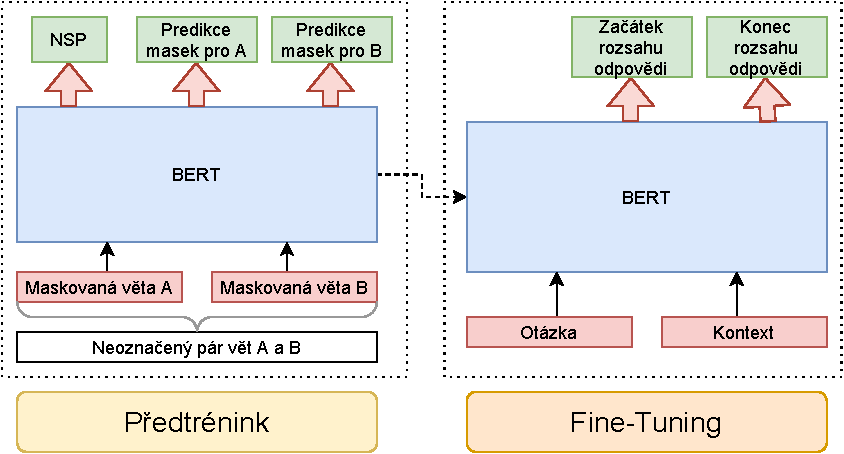
\includegraphics{obrazky/bert_pretraining_fine_tuning.pdf}
	}
	\caption{Vlevo předtrénink enkodéru BERT na úlohách \emph{ML modeling} a \emph{NSP}. Vpravo předtrénovaný model BERT dotrénován na konkrétní úlohu -- odpovídání na otázky. Obrázek byl inspirován obrázkem 1 z článku \cite{BERT}.}
	\label{bert}
\end{figure}

\medskip
\textbf{Maskované modelování jazyka} (ML modeling) 
je úloha velmi podobná již dříve zmíněné úloze predikce následujícího slova ve větě. Je ale použit přístup, kdy je určité procento slov v~textu \emph{maskováno}, aby nebyl původní úkol kvůli obousměrné reprezentaci transformerů triviální.\par
Při tréninku je 15 \% slov každé věty nahrazeno tokenem [MASK], jehož původní význam je poté na základě okolního kontextu hádaný \cite{BERT}. Pro tento úkol je na enkodér napojena klasifikační vrstva, pomocí které je určena pravděpodobnost pro každé slovo ve slovníku, jež by mohlo token [MASK] nahradit.\par
\smallskip
\textbf{Predikce následující věty} (NSP) je druhým typem úlohy pro předtrénink modelu BERT. Jeho snahou je naučit model porozumět vztahu nejen mezi jednotlivými slovy, ale taky mezi významem celých vět.\par
Trénovací datová sada je rozdělena na dvojice vět A~a B. Model má za úkol předpovědět, je-li věta B větou navazující na větu A~v~kontextu. V~50 \% případů je věta B opravdu větou následující. Ve zbytku je to náhodně zvolená věta z~korpusu.\par
Práce \cite{BERT} také uvádí, že navzdory jednoduchosti tohoto úkolu je jeho přínos pro pozdější aplikaci modelu pro odpovídání na otázky velký.\par

\paragraph{Formát vstupu}
modelu BERT je koncipován tak, aby mohl být použit pro větší spektrum aplikací, pro které je zamýšlen. Proto je umožněno na vstupu pomocí jediné sekvence tokenů reprezentovat jak jednu, tak i dvě vstupní sekvence, jako třeba otázku a~odpověď.

\begin{figure}[hbt]
	\centering
	\scalebox{0.45}{
	    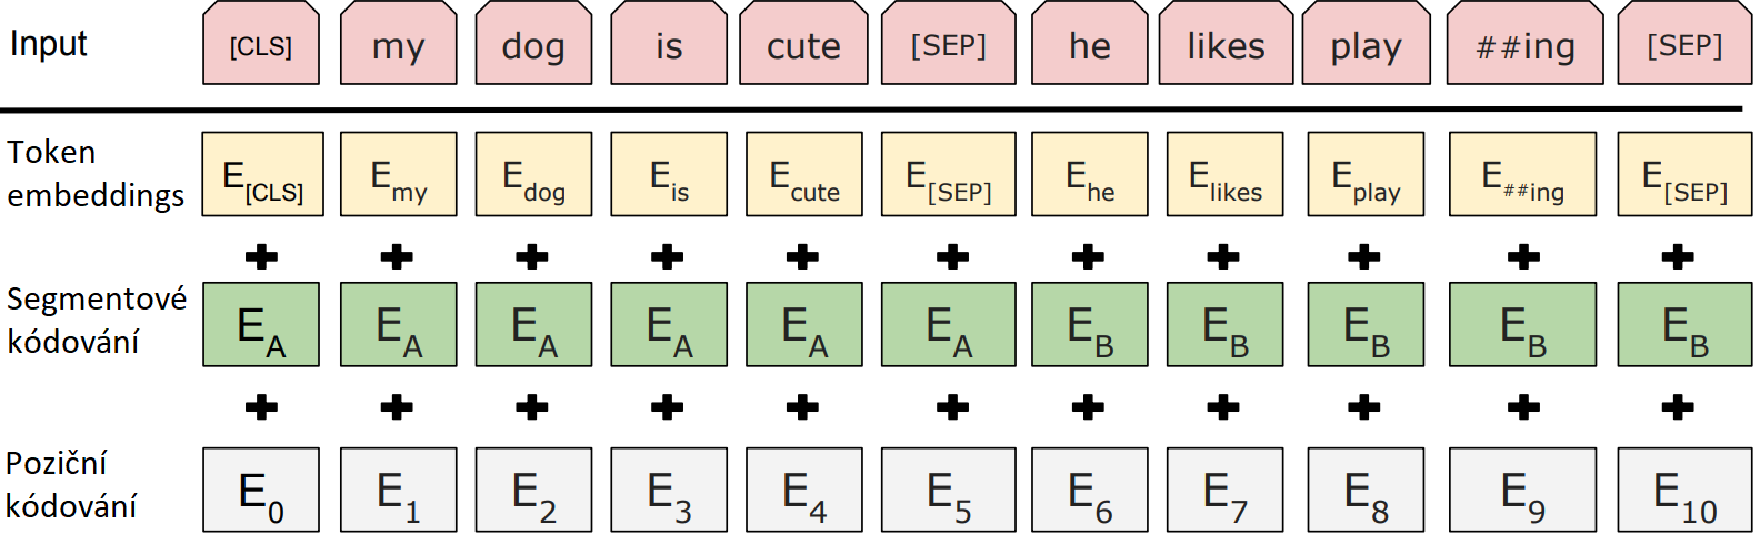
\includegraphics{obrazky/bert_input_new.pdf}
	}
	\caption{Příklad formátu vstupu \uv{\emph{input}} modelu BERT převzatý z \cite{BERT}. Znázorněno je: poziční (\emph{position}), segmentové a~token \emph{embeddings} a~speciální tokeny [CLS] a~[SEP].}
	\label{bert_input}
\end{figure}

Pro vektorovou reprezentaci tokenů jsou použity Wordpiece embeddings~\cite{wordpiece}, popsané v~\ref{wordpiece_embb}. K~těm je přidáno poziční kódování, kvůli použití architektury transformer a~segmentové kódování, které identifikuje, které sekvenci vstupu jednotlivé tokeny náleží. Příklad je naznačen na obr. \ref{bert_input}.\par
Pro popis vstupu jsou navíc použity dva speciální tokeny [CLS] a~[SEP]. Token [CLS] je přidán vždy na začátek vstupu, token [SEP] je přidán na konec každé sekvence. Token [CLS] je využit také jako výstup pro klasifikační úlohy (například předtrénink na NSP).

\subsection{ALBERT}
Informace v~této podkapitole jsou převzaty ze článku \cite{ALBERT} -- \emph{A~Lite BERT for self-supervised learning of language representations}.\par
Hlavním problémem modelu jako BERT je jeho velikost -- asi 110 milionů parametrů v~jeho základní verzi. Zvětšováním modelu se většinou dá dosáhnout zlepšení, je to však problém kvůli omezené paměti grafických karet a~množství času potřebného pro trénink.\par
\textbf{ALBERT} -- A~Lite BERT, je model představený v~roce 2019 článkem \cite{ALBERT}. Vychází z~modelu BERT a~dosahuje lepších výsledků na datových sadách pro porozumění textu, přestože má mnohem menší počet parametrů, než velká verze modelu BERT. V~následujících odstavcích jsou shrnuty hlavní přínosy modelu ALBERT.

\paragraph{Faktorizace parametrů reprezentací} -- \emph{Factorized embedding parameterization}\\ 
\emph{Wordpiece embeddings} se učí reprezentovat tokeny nezávisle na kontextu, zatímco skryté vrstvy modelu se učí reprezentaci závislou na kontextu. Zvětšení velikosti skryté vrstvy způsobí u~modelu BERT stejný nárůst velikosti reprezentace tokenů, jejichž význam není tak podstatný a~model to zbytečně zatěžuje.
Díky odstranění provázanosti velikosti dimenze \emph{wordpiece embeddings} a~dimenze skryté vrstvy modelu je možno lépe zvětšovat velikost skrytých vrstev bez toho, aby to ovlivnilo velikost reprezentací ve slovníku.

\paragraph{Sdílení parametrů mezi vrstvami} -- \textit{Cross-layer parameter sharing}\\
Parametry napříč vrstvami jsou sdíleny, což zamezuje růstu počtu parametrů při zvětšování hloubky modelu a~způsobuje jejich efektivnější využití. Ve výsledku má velká verze modelu ALBERT mnohonásobně méně parametrů, než velká verze modelu BERT.

\paragraph{Trénink návaznosti dvou vět} -- \textit{Inter-sentence coherence loss}\\
Trénink modelu BERT pomocí predikce následující věty (NSP) se částečně překrýval s~úkolem predikce maskovaného tokenu, protože mohla být nesouvislost vět odhadnuta na základě nepříslušnosti slov ke stejnému tématu.\par
Pro trénink modelu ALBERT je pro tento úkol použita stejná dvojice vět A~a B, u~kterých se určuje, zda B navazuje na A. Při nenávaznosti však není věta B náhodně vybrána z~jiného korpusu, ale je pouze prohozena s~větou A. Model je tak lépe schopen naučit se logickou souvislost vět, místo odhadu tématu, ke kterému se věty vztahují bez toho, aby na sebe logicky navazovaly.
\bigskip\bigskip
\paragraph{ALBERT (resp. BERT) pro odpovídání na otázky}
Pro využití modelu ALBERT (resp. BERT) na konkrétní úkoly vyžadující porozumění textu je potřeba provést \emph{naladění} modelu.\par
Pro odpovídání na otázky je na výstup modelu napojena lineární vrstva, která je natrénována na určení indexu začátku a~konce odpovědi v~rámci celé vstupní sekvence. Pro začátek a~konec je poté vybrána validní\footnote{Podmínky jako: start idx < end idx, nebo to, že se odpověď se nenachází v~první sekvenci (otázce).} dvojice indexů, označující rozsah odpovědi.\par
Pro naladění na daný úkol jsou optimalizovány parametry lineární klasifikační vrstvy i enkodéru ALBERT (resp. BERT), nebo pouze lineární vrstvy (což vyžaduje mnohem kratší trénink).

%=========================================================================
%===============================================================================

\chapter{Řazení dokumentů dle relevance}
\label{document_indexing}
Tato kapitola popisuje metody pro indexaci a~řazení dokumentů dle relevance, které jsou využity při vyhledávání relevantního dokumentu, rozebraném v~části \ref{retriever_imp}. Nejprve je vysvětlen význam indexu v~kontextu řazení dokumentů a~poté algoritmy, které jej využívají k~vyhledávání. Nakonec jsou diskutovány problémy velké báze dat, jako je Wikipedie.\par
Informace v~této kapitole jsou čerpány z~prezentací stanfordského kurzu \emph{Information Retrieval and Web Search} \cite{stanford:retrieval} a~knihy \emph{Introduction to Information Retrieval} \cite{information_retrieval}.

\section{Indexování dokumentů}
Pro vyhledávání dokumentů s~použitím webových zdrojů jako Wikipedie jsou typické rozsáhlé texty, které by bylo náročné procházet sekvenčně. Proto je důležité vytvořit strukturu, která je dále použita metodami pro řazení dokumentů a~umožní optimalizované vyhledávání. Taková struktura se nazývá \textbf{index}.\par
Index poskytuje informace o~výskytu jednotlivých termů v~prohledávaných dokumentech a~je vytvořen ještě před začátkem vyhledávání. Nejpoužívanější variantou je tzv. \emph{invertovaný index}.\par
Před vytvořením indexu je užitečné provést co nejlepší normalizaci prohledávaných dokumentů. Metody pro zpracování textu byly podrobně popsány v~kapitole \ref{preprocessing} (převod na malá písmena, lemmatizace, odstranění stop slov).\par
\textbf{Invertovaný index} je struktura obsahující všechna slova (termy) prohledávaného korpusu. Pro každý term je uložen seznam dokumentů (označených \emph{docID}), které daný výraz obsahují. Může obsahovat doplňující informace o~počtu výskytů termu v~dokumentu, případně přesné pozice. Informace jsou poté využity při řazení dokumentů, tzv. \emph{ohodnoceném vyhledávání}.

\subsection{Úskalí velké báze dat jako Wikipedie}
Česká Wikipedie obsahuje velké množství článků (asi 3,5\,GB v~nekomprimované podobě). Pro prohledávání celé Wikipedie je potřeba vytvořit a~udržovat index, což je pro takový objem dat poměrně výpočetně a~paměťově náročné. Je složité pomocí běžných nástrojů sestavit index pro celou Wikipedii.\par
Dalším problémem je různá délka dokumentů, nestrukturovanost některého textu a~dynamicky se měnící prostředí, kdy jsou články na Wikipedii pravidelně aktualizovány.\par\enlargethispage{\baselineskip}
Způsoby prohledávání Wikipedie a~vypořádání se se zmíněnými problémy jsou popsány podkapitole \ref{design} a~kapitole \ref{chapter:implementace}, věnované implementaci.

%=========================================================================
\section{Ohodnocené vyhledávání pro řazení dokumentů}
Při dotazování na vytvořený index nestačí pouze výčet dokumentů, které termy přítomné v~dotazu obsahují. Ohodnocené vyhledávání umožňuje (pomocí speciálních vztahů) získání množiny seřazených \emph{n} nejvíce relevantních dokumentů.\par

\subsection{TF-IDF (Term frequency -- Inversed document frequency)}
\label{tf-idf}

\textbf{Četnost termu} (TF -- rovnice \ref{tf_eq}) je počet výskytů vyhledávaného termu v~daném dokumentu. Vycházíme z~předpokladu, že dokument s~deseti výskyty termu je pro dotaz relevantnější, než dokument obsahující vyhledávaný term pouze jednou. Neznamená to však, že je dokument $10\times$  relevantnější -- růst relevance není přímo úměrný TF.\par
Jednotlivé termy nenesou stejnou informační hodnotu (např. stop slova \ref{stopwords}) a~ojedinělé výrazy jsou často zásadní pro relevanci k~dotazu (což souvisí i s~neúměrným růstem relevance s~růstem TF).\par

\begin{equation}
\label{tf_eq}
    TF_{t,d} = log(1+tf_{t,d})
\end{equation}

\textbf{Dokumentová četnost} (DF) je počet dokumentů, které obsahují vyhledávaný term. Účelem je identifikace termů, vyskytujících se jenom ve zlomku dokumentů, které nejspíš ponesou zásadní informační hodnotu. Cílem je zohlednit nepřímou úměru závislost růstu relevance dokumentu a~četnosti termu. Převrácená dokumentová četnost  (IDF -- viz rovnice~\ref{idf_eq}) dělí celkový počet dokumentů \emph{N} dokumentovou četností pro daný term. Hodnota IDF je tedy vyšší pro vzácnější termy.\par

\begin{equation}
\label{idf_eq}
    IDF_{d} = log(\frac{N}{df_t})
\end{equation}

\textbf{TF-IDF} je statistická metoda, která použitím uvedených dvou metrik hodnotí relevanci dokumentu.
Pro výpočet váhy TF-IDF pro daný term \emph{t} v~dokumentu \emph{d} platí tedy:

\begin{equation}
    \text{TF-IDF}_{t,d} = TF_{t,d} \cdot IDF_d
\end{equation}

Ohodnocení \emph{S} dokumentu \emph{d} pro dotaz \emph{q} je potom sumou jednotlivých ohodnocení termů \emph{t} dané otázky \emph{q}.

\begin{equation}
    S(q,d) = \sum_{t\in{q \cap d}}^{}\text{TF-IDF}_{t,d}
\end{equation}

\subsection{BM25 (Best Match 25)}
\label{bm25}
Skóre BM25 (označované také jako Okapi) bylo představeno v~\cite{bm25}. Jedná se o vylepšení klasické hodnotící funkce TF-IDF, které využívá poznatky statistiky a~pravděpodobnosti pro řazení dokumentů dle jejich relevance s~ohledem na vztah délky dokumentu a~četnosti výskytů termu v~něm.\par
Delší dokumenty budou mít pravděpodobně větší $tf_{t,d}$. To je potřeba ve výsledném ohodnocení zohlednit, aby nebyly delší dokumenty nutně zvýhodněny.
Výsledný vzorec pro ohodnocení dokumentu \emph{d} pomocí BM25 vzhledem k~otázce \emph{q} je:
\begin{equation}
    S(q,d)^{BM25} = \sum_{t \in q} \left(IDF_d \cdot \frac{(k_1+1)\cdot tf_t}{k_1\cdot ((1-b)+b \cdot \frac{dl}{avdl}) + tf_t}\right),
\end{equation}
kde $tf$ a~$idf$ jsou metriky vysvětlené v~podkapitole \ref{tf-idf}, $dl$ je délka dokumentu $d$, $avdl$ je průměrná délka dokumentu v~kolekci a~$b,k_1$ jsou konstanty:
\begin{itemize}
    \item $k_1$ ovlivňuje dopad \emph{TF} na výsledné skóre dokumentu. Obvykle je volena v~rozmezí $k_1\in(1,2\,;\,2)$. Pro nízké hodnoty $k_1$ roste význam dokumentu s~rostoucí \emph{TF} poměrně rychle.
    \item $b$ ovlivňuje normalizaci délky dokumentu, obvykle je volena hodnota $b=0,75$. Hodnota $b=1$ znamená úplnou a~$b=0$ žádnou normalizaci délky dokumentu.
\end{itemize}

Výhodu hodnotící funkce BM25 oproti obyčejnému TF-IDF lze demonstrovat na následujícím příkladě.\\ \medskip
Mějme vyhledávaný dotaz \uv{\emph{term frequency}} a~dva dokumenty $d_1$ a~$d_2$:\par

\begin{table}[H]
\centering
\begin{tabular}{|c|l|l|}
\hline
      & term & frequency \\ \hline
$d_1$ & 1024 & 1         \\ \hline
$d_2$ & 16   & 8         \\ \hline
\end{tabular}
\begin{tabular}{|c|l|l|}
\hline
      & \textbf{TF-IDF} & \textbf{BM25} \\ \hline
$d_1$ & \textbf{87} & 31         \\ \hline
$d_2$ & 75 & \textbf{43}         \\ \hline
\end{tabular}
\caption{Výskyt termů \uv{term} a~\uv{frequency} v~dokumentech $d_1$ a~$d_2$ a~ohodnocení jednotlivých dokumentů podle funkcí TF-IDF a~BM25 ($k_1 = 2$)}
\label{tab:tf}
\end{table}

Tabulka \ref{tab:tf} ukazuje, jak BM25 lépe zohlednilo počet výskytů termů a~skutečně ohodnotilo lépe relevantnější dokument.\par \medskip
Pro BM25 existují také modifikace, jako BM25+ \cite{bm25_too_long}, BM25L \cite{bm25_plus} a~další, které se snaží vypořádat se znevýhodněním příliš dlouhých dokumentů klasickou funkcí BM25. Byly porovnány v~\cite{bm25_improvements}. Závěr toho článku ale ukazuje, že neexistuje modifikace, která by systematicky zlepšila dosažené výsledky vyhledávání ve všech případech.\par

\subsection{DPR (Dense Passage Retrieval)}
\label{dpr}
DPR je technika, představená článkem \cite{dpr}, která využívá architekturu dvou enkodérů. Pomocí jednoho z enkodérů je  každý dokument převeden na vektorovou reprezentaci. Z~těch je sestaven vyhledávací index. Druhý enkodér je určen pro získání reprezentace otázky. Pro vektor otázky je poté nalezen dokument (nebo více dokumentů), jehož vektor je vektoru otázky nejblíže (rovnice~\ref{similarity}).\par
\begin{equation}
    \label{similarity}
    sim(q,d) = E_Q(q)\cdot E_D(d)
\end{equation}
V rovnici \ref{similarity} \cite{dpr} je $sim(q,d)$ skóre relevance otázky $q$ a dokumentu $d$, $E_Q$ je enkodér použitý pro reprezentaci otázky a $E_D$ pro reprezentaci dokumentu.\par
Jako enkodéry jsou použity modely BERT (je tomu tak v \cite{dpr}, ale stejně je tomu také např. v \cite{fajcik2021pruning} pro implementaci systému R2-D2). Ty jsou trénovány tak, aby po výpočtu blízkosti vektorů otázky a relevantních pasáží měly relevantní pasáže co nejmenší vzdálenost.

%=========================================================================
%===============================================================================

\chapter{Dostupné datové sady a~výběr}
\label{available_datasets}
Tato kapitola se zabývá popisem a~výběrem datových sad (datasetů) pro realizaci a~evaluaci systému.\par
Datová sada je v~oblasti strojového učení velká anotovaná kolekce dat pro trénink a~vyhodnocování neuronových sítí nebo celých systémů. Obvykle obsahuje pro každý příklad vstupní data a~jejich anotaci.\\
Datové sady je možno rozdělit podle toho, v~jaké fázi vývoje s~nimi pracujeme.
\begin{itemize}
    \item \textbf{Trénovací (train)} Používá se pro naučení neuronové sítě. Při zpracovávání trénovací datové sady se model učí a~upravuje své parametry. Na konci tréninku může model konvergovat ke 100\% úspěšnosti na trénovací datové sadě.
    \item \textbf{Validační (dev)} Slouží pro průběžné vyhodnocení existujícího modelu při vývoji. Model se z~validačních dat neučí. Může být využita například k~úpravě hyperparametrů nebo zastavení tréninku modelu, když se jeho úspěšnost na validační datové sadě přestane zlepšovat. Vytvořena může být vybraným zlomkem trénovacího datasetu nepoužitým pro trénink.
    \item \textbf{Testovací (test)} Obsahuje příklady z~reálného světa, na kterých je model/systém vyhodnocen po dokončení jeho vývoje. Testovací dataset je často shodný s~validačním.
\end{itemize}
Pro trénink neuronových sítí pro odpovídání na otázky by měla datová sada obsahovat hlavně:
\begin{itemize}
    \item otázku
    \item kontext (dokument obsahující odpověď)
    \item odpověď
    \item případně doplňující informace (jako začátek odpovědi, délku odpovědi apod.)
\end{itemize}
Vytvoření takové datové sady je složitý úkol, vyžadující velké množství lidských zdrojů. Je potřeba nasbírat dostatečné množství dokumentů, pro které někdo musí vymyslet otázky a~vyznačit v~dokumentech příslušné odpovědi. Tvorba datových sad obvykle probíhá pomocí \emph{crowdsourcingu}\footnote{\emph{Crowdsourcing} označuje proces získání potřebné služby, nápadů, příspěvků, či pomoci při řešení problémů, od velké skupiny lidí. (\url{https://wikisofia.cz/wiki/Crowdsourcing} [cit. 22-03-2021])}.

%=========================================================================
\section{Datové sady pro angličtinu}
Pro angličtinu existuje celá řada datových sad zaměřených na odpovídání na otázky. Nejznámější z~nich je  SQuAD (\emph{Stanford Question Answering Dataset}) \cite{squad}. Dataset obsahuje asi 100 000 anotovaných dvojic otázka\,--\,odpověď z~více než 500 různých článků z~anglické Wikipedie. Existuje také rozšířená verze tohoto datasetu. SQuAD~2.0 \cite{squad_v2} obsahuje navíc 50 000 otázek, na které v~ přiloženém kontextu neexistuje odpověď. Pokud tedy dokument odpověď neobsahuje, model to musí umět určit.\par
Další datasety jsou například NQ (Natural Questions) se zaměřením na otevřenou doménu nebo HOTPOTQA, vyžadující pro zodpovězení otázky spojování informací z více dokumentů. Čeština takovou diverzitou datových sad nedisponuje.

%=========================================================================
\section{Datové sady pro češtinu}
Čeština nabízí poměrně omezené zdroje\footnote{Co se týká datasetů pro odpovídání na otázky, existuje pouze zmíněný SQAD. Angličtina nabízí datasety specializované např. pro otevřenou doménu.} oproti anglickým datovým sadám.\par 
Nejznámější je datová sada SQAD (Simple Question Answering Database) \cite{sqad}. Obsahuje přes 13 000 příkladů otázek s~odpovědí v~přiloženém kontextu, pocházejícího z~české Wikipedie. Datová sada obsahuje otázky směřované na časový údaj, entitu, lokaci, osobu atd., včetně 16 \% otázek typu ano/ne. Velikost datasetu je přesně popsána v tabulce \ref{tab:sqad_size}.\par
Existuje také česká verze anglického datasetu SQuAD, prezentovaná v~práci \cite{czech_squad}. Datová sada je strojovým překladem původního datasetu SQuAD 1.1 a~SQuAD2.0. Oproti anglické verzi však obsahuje asi 70 000 otázek pro první (1.1) a~110 000 otázek pro druhou (2.0) verzi datové sady SQuAD (tabulka \ref{tab:squad_size}). Ztráta části rozsahu datové sady je způsobena problémy s~vyznačením odpovědi ve strojově přeložené verzi dokumentu.

%=========================================================================
\section{Výběr trénovacích a~testovacích dat}
\label{dataset_choice}
Pro systém je potřeba vybrat data pro natrénování modelů pro extrakci odpovědi a~pro validaci výsledného systému.\par
Pro trénink anglického modelu byl vybrán anglický SQuAD 1.1 a 2.0 (obsahující i validační část datasetu). Po zvážení bylo rozhodnuto o použití a porovnání obou verzí datasetu. Testovací data obsahují pouze otázky, pro které existuje nad otevřenou doménou odpověď, a je tedy porovnáno, která verze datasetu byla pro trénink readeru vhodnější.\par
Pro trénink českého (vícejazyčného) modelu byl vybrán český překlad anglického datasetu SQuAD 1.1 a 2.0 \cite{czech_squad} kvůli jeho velikosti a~porovnatelnosti s~anglickou verzí datasetu.\par
\medskip
Jako testovací datová sada byl zvolen český dataset SQAD v3.0, ze kterého bylo odstraněno 16 \% otázek, očekávajících odpovědi ano/ne. Datová sada nejlépe odpovídá reálnému scénáři užití systému, protože obsahuje otázky a~odpovědi z~článků české Wikipedie (na rozdíl od trénovacích datasetů).\par
V době použití byly zjištěny velikosti datových sad, které jsou uvedeny v tabulce \ref{tab:squad_size_new} (neodpovídají přesně informacím z původního článku).

\begin{table}[H]
    \centering
    \begin{tabular}{|c|r|r|r|}
        \hline
        \multicolumn{2}{|l|}{Dataset}         & \begin{tabular}[c]{@{}l@{}}Anglické\\  otázky\end{tabular} & \begin{tabular}[c]{@{}l@{}}České \\ otázky\end{tabular} \\ \hline \hline
        \multirow{2}{*}{\textbf{SQuAD 1.1}} & Trénink  & 87,599                                                     & 64,164                                                  \\ \cline{2-4} 
                                   & Validace & 10,570                                                     & 8,739                                                   \\ \hline
        \multirow{2}{*}{\textbf{SQuAD 2.0}} & Trénink  & 130,319                                                    & 107,088                                                 \\ \cline{2-4} 
                                   & Validace & 11,873                                                     & 10,845                                                  \\ \hline
        \end{tabular}
        \caption{Velikost datasetů SQuAD 1.1 a~2.0 pro češtinu a~angličtinu podle \cite{czech_squad}.}
    \label{tab:squad_size}
\end{table}

\begin{table}[H]
\centering
\begin{tabular}{|c|r|r|r|}
\hline
\multicolumn{2}{|l|}{Dataset}         & \begin{tabular}[c]{@{}l@{}}Anglické\\  otázky\end{tabular} & \begin{tabular}[c]{@{}l@{}}České \\ otázky\end{tabular} \\ \hline \hline
\multirow{2}{*}{\textbf{SQuAD 1.1}} & Trénink  & 88,638                                                     & 69,169                                                  \\ \cline{2-4} 
                           & Validace & 10,808                                                     & 9,615                                                   \\ \hline
\multirow{2}{*}{\textbf{SQuAD 2.0}} & Trénink  & 131,958                                                    & 115,415                                                 \\ \cline{2-4} 
                           & Validace & 12,171                                                     & 12,066                                                  \\ \hline
\end{tabular}
\caption{Velikost datasetů SQuAD 1.1 a~2.0 zjištěná při jejich použití.}
\label{tab:squad_size_new}
\end{table}

\section*{Úskalí datasetu SQAD}
Dataset SQAD má pro vyhodnocení systému nad otevřenou doménou podobné nevýhody jako SQuAD. Otázky jsou přímo vázané ke konkrétnímu článku, z čehož vyvstávají problémy pro jejich jiné využití.\par 
Některé otázky nemusí dávat bez přiloženého kontextu smysl, a je tedy nemožné (nebo velmi obtížné) pro ně najít odpověď. Některé mohou být také nejednoznačné a správných odpovědí pro ně může být bez kontextu několik, v datasetu se však nachází jako referenční pouze jediná, která je extrakcí z přiloženého kontextu. \par 
Dalším z možných problémů je také vázanost datasetu na časové období, kdy byl vytvořen/zveřejněn (2019). Příkladem může být otázka \uv{Kolik evropských států tvoří Evropskou unii?}, pro kterou už odpověď \uv{28} není realitou (viz Brexit).\par
Procházet ručně a vybrat pro odstranění takové otázky z datové sady je pro jednoho člověka náročné, a proto to je případně zohledněno až při lidském vyhodnocení zmíněném v části \ref{metriky}.

\begin{table}[H]
\centering
\begin{tabular}{|l|l|l|}
\hline
Dataset            & počet záznamů & bez ano/ne      \\ \hline
\textbf{SQAD v3.0} & 13,476        & \textbf{11,273} \\ \hline
\end{tabular}
\caption{Velikost datasetu SQAD v3.0 při jeho použití pro vyhodnocení systému.}
\label{tab:sqad_size}
\end{table}

%=========================================================================
%===============================================================================

\chapter{Návrh systému a~jeho komponent}
\label{chapter:design_}
V~této kapitole je rozebrán návrh systému, než přijde popis implementace jeho jednotlivých částí (v kapitole \ref{chapter:implementace}). Nejprve je popsán generický koncept systému pro odpovídání na otázky, zvolený přístup k~řešení a~motivace za finálním návrhem. Následuje rozdělení problému na části a~jejich návrh včetně popisu blokových schémat hlavních komponent. Diskutován je návrh vyhodnocení výsledného systému v kontextu otevřené domény. Na závěr kapitoly je zmíněno několik existujících řešení.

\begin{figure}[hbt]
	\centering
	\scalebox{1.2}{
	    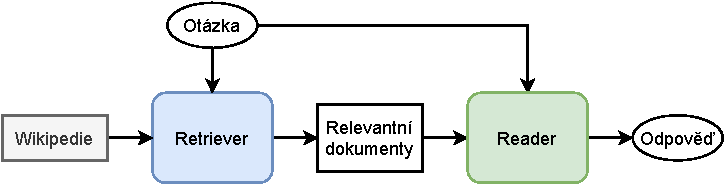
\includegraphics{obrazky/reader-retriever-scheme.pdf}
	}
	\caption{Generické schéma (prezentované například v~\cite{drQA}) open-domain QA systému}
	\label{qa_scheme}
\end{figure}

%=========================================================================
\section{Zvolený přístup k~problému}
Odpovídání na otázky nad otevřenou doménou (open-domain QA) má obvykle dvě hlavní (na sobě téměř nezávislé) části, jak je naznačeno na obrázku \ref{qa_scheme}. První částí je \emph{Retriever}, který má za úkol získat z~internetu (pro nás z~Wikipedie) relevantní dokumenty, které by mohly obsahovat odpověď na danou otázku. Druhým blokem je \emph{Reader}, který provádí extrakci odpovědi ze získaného kontextu \cite{drQA}.\par
\noindent\emph{Retriever} části systému je věnována pozornost v~podkapitole \ref{retriever_imp}.\par
Pro návrh systému byla největším dilematem realizace \emph{Reader} části systému pro kvalitní extrakci odpovědi v~češtině. Chtěl jsem využít některého z~populárních předtrénovaných modelů (\ref{bert_albert}) založených na Transformers \cite{Transformers} architektuře (\ref{transformers}). Proto jsem se rozhodl vyzkoušet přístup, kdy je nativně anglickému ALBERT modelu, který dosahuje špičkových výsledků\footnote{Žebříček nejúspěšnějších modelů dostupný z: \url{https://rajpurkar.github.io/SQuAD-explorer/}}, strojově přeložen získaný dokument i otázka z~češtiny do angličtiny.\par
Pro porovnání jsem zvolil pro extrakci odpovědi vícejazyčný model BERT (m-BERT\footnote{\url{https://github.com/google-research/bert/blob/master/multilingual.md} -- Zjednodušeně řečeno je to model BERT předtrénován na korpusech mnoha jazyků.}), který podporuje 104 světových jazyků s~nejrozsáhlejší Wikipedií. \emph{Fine-tuning} je proveden na českém překladu datové sady SQuAD 1.1 a 2.0 \cite{czech_squad} \cite{squad}. Výsledný systém využívá variantu, která se osvědčila v experimentech jako nejúspěšnější (viz kapitola \ref{system_evaluation}).\par

%=========================================================================
\section{Návrh jednotlivých částí systému}
\label{design}
V~této podkapitole je popsán návrh systému, tedy hlavně \emph{Retrieveru} a \emph{Readeru}. Diskutován je také návrh vyhodnocení systému na datasetu SQAD v3.0.

\subsection{Návrh Retrieveru}
Získání \emph{n} relevantních dokumentů kandidujících pro zodpovězení otázky vyžaduje několik na sebe navazujících kroků (obrázek \ref{retriever-simple-scheme}). V~návrhu a~implementaci jsou použity metody předzpracování textu a~řazení dokumentů popsané v~kapitolách \ref{text_processing} a~\ref{document_indexing}.\par
Retriever dostává na vstupu otázku, která je také hlavním vstupem do celého systému. Dříve, než se na základě otázky začnou přímo prohledávat odstavce české Wikipedie, je dobré z~otázky získat co nejvíce informací, které by mohly vést k těm \emph{správným článkům}. Až po jejich získání jsou jednotlivé články rozděleny na odstavce, které jsou řazeny.\par
\noindent K~získání článku jsou použity tři metody:
\begin{itemize}
    \item \textbf{základní Wiki Search} nezpracované otázky, který někdy přináší uspokojivé výsledky, ale většinou je nedostačující,
    \item \textbf{získání relevantního titulku článku} (pomocí BM25 \ref{bm25}) z~\emph{dumpu} titulků a~abstraktů české Wikipedie\footnote{\url{https://cs.wikipedia.org/wiki/Wikipedie:St\%C3\%A1hnut\%C3\%AD_datab\%C3\%A1ze}} po lemmatizaci otázky a~odstranění stop slov,
    \item \textbf{rozpoznání (pojmenované) entity} v otázce, která by se mohla vyskytovat v~titulku článku a~usnadnit tím \emph{Wiki Search}.
\end{itemize}
Tímto je tedy získán seznam článků z~Wikipedie, který je následně upraven tak, aby se v~něm každý získaný článek vyskytoval pouze jednou.\par
Jednotlivé články je následně třeba rozdělit na odstavce, normalizovat jejich délku, lemmatizovat je, odstranit stop slova a~vytvořit jejich index. Odstavce jsou poté seřazeny hodnotící funkcí BM25 a~z~nich vybrány první \textit{tři}\footnote{V tomto případě pro účely experimentů -- nejúspěšnější varianta je vyhodnocena také s použitím hodnot 5, 8 a 10.} s nejlepším skóre. Pro vyhledávání mezi odstavci je použita lemmatizovaná otázka s~odstraněnými stop slovy. Tři nejvhodnější odstavce jsou získány v~jejich původní, nezpracované podobě a~případně (při použití nativně anglického \emph{readeru} ALBERT) jsou včetně otázky přeloženy do angličtiny.

\begin{figure}[hbt]
	\centering
	\scalebox{0.9}{
	    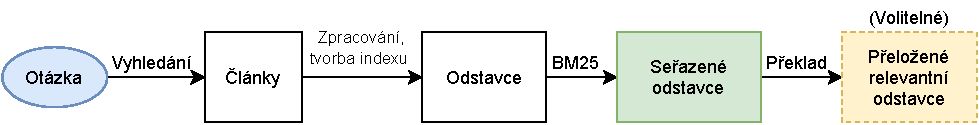
\includegraphics{obrazky/retriever-simple-scheme.pdf}
	}
	\caption{Zjednodušené schéma \emph{retriever} části systému}
	\label{retriever-simple-scheme}
\end{figure}

Následuje podrobný návrh struktury \emph{retrieveru} znázorňující podrobně jednotlivé komponenty na obrázku \ref{retriever-podrobne}.

\begin{figure}[hbt]
    \centering
	\scalebox{0.9}{
	    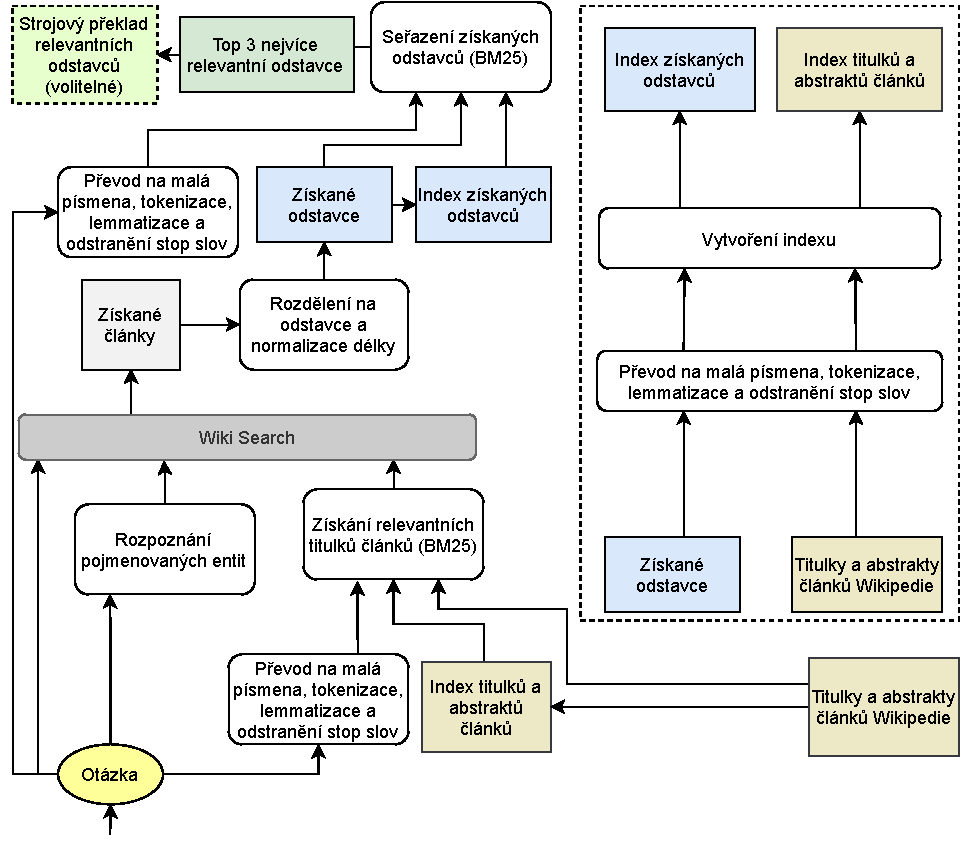
\includegraphics{obrazky/retriever_podrobne.pdf}
	}
	\caption{Podrobné schéma \emph{retriever} části systému}
	\label{retriever-podrobne}
\end{figure}

\subsection{Návrh Readeru}
Část systému pro extrakci odpovědi ze získaného dokumentu byla navržena ve dvou variantách.
\begin{itemize}
    \item \textbf{Anglický ALBERT} s~lineární klasifikační vrstvou pro určení začátku a~konce odpovědi, pro který jsou vstupní dokumenty a~otázka strojově přeloženy do angličtiny. Výsledná odpověď je přeložena opět zpět do češtiny.
    \item \textbf{Vícejazyčný BERT (m-BERT)} opět s~lineární klasifikační vrstvou pro určení začátku a~konce odpovědi, který dokáže odpovídat přímo v češtině.
\end{itemize}
Pro obě varianty je postup získání odpovědi (až na překlad pro anglický ALBERT, který je však součástí \emph{retrieveru}) shodný.\par
Model dostane k~přečtení tři nejvíce relevantní odstavce získané \emph{retrieverem}. Pro každý odstavec je provedena extrakce odpovědi, kdy je vybrána vždy právě jedna validní odpověď s~největším \uv{skóre} (nenormalizovaná logaritmická pravděpodobnost) pro daný dokument. Ze získaných odpovědí je vybrána ta, kterou si je model nejvíce jistý (ta s~největším skóre) a~případně (při použití ALBERT modelu) přeložena zpět do češtiny.\par
\noindent Ostatní odpovědi jsou také uloženy -- pro získání statistických dat při vyhodnocení. \emph{Reader} tak vybere kromě odpovědi také dokument/odstavec, ze kterého je odpověď získána. Může tak být použit pro získání některých dalších informací/kontextu uživatelem.\par
Schéma \emph{readeru} pro extrakci finální odpovědi je naznačeno na obrázku \ref{reader_schema}. Modely, které byly použity k~implementaci a~jsou naznačeny v~návrhu byly blíže popsány v~kapitole~\ref{language_comprehension}, konkrétně v~podkapitole \ref{bert_albert}.

\begin{figure}[hbt]
	\centering
	\scalebox{1.3}{
	    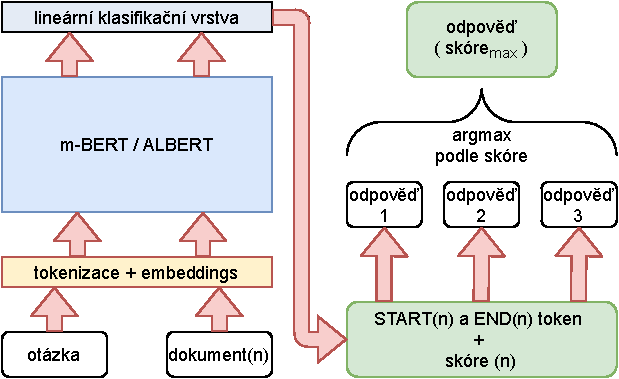
\includegraphics{obrazky/reader_navrh.pdf}
	}
	\caption{Schéma \emph{readeru} (kombinovaně pro oba navržené systémy) pro 3 relevantní dokumenty, kde $n \in (1,3)$. Pro model ALBERT by musel proběhnout ještě strojový překlad finální odpovědi do češtiny.}
	\label{reader_schema}
\end{figure}

\subsection{Návrh vyhodnocení}
Pro vyhodnocení byl vybrán český dataset SQAD v3.0, jak už bylo několikrát zmíněno. Pro vyhodnocení musely být navrženy metriky respektující charakteristiku datové sady i to, že se pohybujeme v~rámci otevřené domény. Kromě tradičních metrik EM (\emph{exact match}) a~F1 (popsány blíže v~kapitole \ref{metriky}) jsem se při návrhu vyhodnocení systému snažil respektovat několik věcí:
\begin{itemize}
    \item Kvůli otevřené doméně může být odpověď nalezena z~jiného kontextu, v~jiném tvaru.
    \item Potřebujeme metriku pro ohodnocení samotného \emph{retrieveru} v~úspěšnosti nalezeného dokumentu.
    \item Metriku pro zohlednění správných odpovědí, které byly nalezeny, i když nebyly vybrány \emph{readerem} jako nejvhodnější.
\end{itemize}
Pro podrobnější popis zvolených metrik viz \ref{metriky}. Metriky jsou použity pro porovnání variant systému i vyhodnocení jeho výsledné verze.

\section{Existující systémy pro otevřenou doménu}
\label{existing_work}
Příkladem existujícího systému pro QA nad otevřenou doménou může být třeba dříve zmíněný článek \cite{drQA} (DrQA) prezentující \emph{retriever\,--\,reader framework}. Je poměrně jednoduchý a podobný navrženému systému v této práci. DrQA byl navržen pro odpovídání na otázky nad anglickou Wikipedií a jeho úspěšnost EM na datasetu SQuAD (1.1) je podle \cite{drQA} necelých 30 \%.\par
Novější implementací může být například systém R2-D2 \cite{fajcik2021pruning}, který patřil k nejvíce úspěšným systémům soutěže NeurIPS 2020 \cite{min2021neurips}. R2-D2, neboli \textit{Rank twice -- Read twice}, používá architekturu sestávající ze čtyř částí: \emph{retriever, reranker, }extraktivní a generativní \emph{reader}. Retriever používá DPR \cite{dpr}(popsáno v části \ref{dpr}) a reranker využívá enkodér transformer architektury. Jeho úspěšnost na datasetu NQ (Natural Questions) dosahuje 55 \% EM. V zásadě jsou si state of the art systémy v architektuře retriever\,--\,reader velmi podobné, s drobnými odchylkami (jako je reranker, extraktivní/generativní reader). Implementace \mbox{R2-D2} se navíc snaží omezit paměťovou náročnost modelu. Pro modely bez omezení dosahuje úspěšnost těch nejlepších více jak 60 \% F1 skóre\footnote{Nejlepší výsledky dostupné z: \url{https://ai.google.com/research/NaturalQuestions/leaderboard}}.\par\medskip
Pro češtinu existuje systém AQA (Automatic Question Answering) poprvé prezentován v práci \cite{aqa} a od té doby zdokonalován. Práce \cite{aqa}, poskytující jakýsi benchmark pro evaluaci systému nad otevřenou doménou pro dataset SQAD (v1.0), je z roku 2016. Pozdější vyhodnocení pro zdokonalený systém a dataset SQAD v1.1 z roku 2018 je v článku \cite{aqa2018}. Výsledky systému vyhodnoceného v roce 2018 jsou shrnuty v tabulce \ref{tab:aqa_benchmark}. Novější vyhodnocení systému fungujícího nad otevřenou doménou architektury retriever\,--\,reader pro dataset SQAD 3.0 není k dispozici.
\begin{table}[H]
\centering
    \begin{tabular}{|l|c|c|}
    \hline
    \multicolumn{1}{|c|}{{\textbf{AQA}}} & EM [\%]    & \multicolumn{1}{l|}{počet testovacích vzorků} \\ \hline
    \textbf{SQAD v1.0}                       & 49,83 & 3301                                         \\ \hline
    \textbf{SQAD v1.1}                       & 38,08 & 3301                                         \\ \hline
    \end{tabular}
\caption{Úspěšnost systému AQA v přesné shodě s referenční odpovědí na datových sadách SQAD 1.0 a 1.1.}
\label{tab:aqa_benchmark}
\end{table}

Paralelně s vývojem mého systému vzniká také diplomová práce s názvem \textit{Vícejazyčný systém pro odpovídání na otázky nad otevřenou doménou} (studenta Bc. Michala Slávky pod vedením Ing. Martina Fajčíka). Ta se zabývá tvorbou open-domain systému schopného odpovídat na otázky v 17 jazycích. Pro retriever používá práce taktéž hodnotící funkci BM25. Co se týká readeru, experimentuje práce, podobně jako ta má, s více přístupy. Jeden z nich vyhledává dokumenty pouze v angličtině a využívá strojového překladu původních otázek. Odpověď v angličtině je pak znovu přeložena do původního jazyka. Druhý se zabývá použitím vícejazyčného modelu. Pro reader je použit, na rozdíl od této práce, generativní model T5 a (vícejazyčný) mT5.

\chapter{Implementace a~použité technologie}
\label{chapter:implementace}
Obsahem této kapitoly je výčet použitých nástrojů a~popis implementace jednotlivých částí systému. Je popsáno jak a~pomocí jakých knihoven byl návrh z kapitoly \ref{chapter:design_} realizován a~jaké problémy bylo potřeba vyřešit. Rozebráno je také zpracování dat potřebných pro funkci systému i jeho vyhodnocení.

%=========================================================================
\section{Použité nástroje a~technologie pro implementaci}
\label{pouzite_nastroje}
V této podkapitole jsou popsány technologie a~knihovny použité při implementaci výsledného systému.\par
Pro implementaci byl vybrán jazyk \textbf{Python} (3.7.10), který nabízí největší množství knihoven a~nástrojů vhodných pro realizaci systému. Zároveň je vhodný ke zpracování dat a~je sympatický svou jednoduchou syntaxí. Nabízí také prostředí \emph{Jupyter notebook}, které je velmi pohodlné pro práci s daty a vývoj.\par
Některé knihovny implementují poznatky popsané v kapitolách \ref{text_processing}, \ref{language_comprehension} a~\ref{document_indexing}. Knihovny běžného charakteru, jako je například \texttt{json}, ve výčtu nejsou uvedeny.

\begin{itemize}
    \item \textbf{PyTorch}\footnote{\url{https://pytorch.org/}}
    je open-source framework pro strojové učení, zejména pro zpracování obrazu a~přirozeného jazyka. \par
    Nabízí implementace mnohých druhů neuronových sítí a~tensorových operací s GPU akcelerací (CUDA).
    
    \item \textbf{HuggingFace -- Transformers}\footnote{\url{https://huggingface.co/transformers/}}
    je populární (open-source) implementací nejznámějších Transformers architektur, jako je BERT nebo ALBERT (dále RoBERTa, XLM \dots), vyvinuta společností HuggingFace.\par
    Nabízí nástroje pro jednoduchou práci s modely, předzpracování jejich vstupu, trénink atd. Pro implementace modelů obecného využití jako BERT nabízí také jejich verze pro konkrétní úlohy, jako je odpovídání na otázky (extrakce odpovědi). Pro každou architekturu je k dispozici typicky několik předtrénovaných verzí (BERT base, BERT large \dots), které je možné dotrénovat pro specifický úkol.\par
    
    \item \textbf{HuggingFace -- Datasets}\footnote{\url{https://huggingface.co/docs/datasets/}}
    umožňuje snadnou práci s veřejně dostupnými datasety. Usnadňuje jejich načtení a~efektivní předzpracování.\par 
    Díky dostupnosti zdrojových kódů umožňuje také úpravu skriptu pro načtení jiné datové sady, která doposud v oficiálním seznamu knihovny není dostupná.
    
    \item \textbf{DeepPavlov}\footnote{\url{https://deeppavlov.ai/}}
    je open-source framework, postavený na Pytorch, TensorFlow\footnote{\url{https://tensorflow.org/}} a~Keras, pro usnadnění vývoje a~výzkumu v oblasti zpracování přirozeného jazyka, konkrétně dialogových systémů.
    
    \item \textbf{Rank-bm25}\footnote{\url{https://github.com/dorianbrown/rank\_bm25}}
    je knihovnou implementující hodnotící algoritmy z rodiny BM25 \cite{bm25_improvements} (Okapi, BM25+, BM25L).\par
    Nabízí velmi jednoduché API pro indexaci a~řazení dokumentů.
    
    \item \textbf{NumPy}\footnote{\url{https://numpy.org/}}
    nabízí jako knihovna velmi efektivní operace pro práci s vektory, maticemi a~vícerozměrnými poli. Je nabízena pod licencí BSD (open-source).
    
    \item \textbf{NLTK}\footnote{\url{https://www.nltk.org/}}
    (Natural Language Toolkit) je open-source knihovna nabízející nástroje pro zpracování textu a~přirozeného jazyka.\par Prostřednictvím jednoduchého API umožňuje tokenizaci (včetně dělení na věty), stematizaci, nebo tagování částí textu. 
    
    \item \textbf{MorphoDiTa\footnote{\label{note9}\url{https://ufal.mff.cuni.cz/morphodita}} (corpy)\footnote{\url{https://corpy.readthedocs.io/en/stable/api/morphodita.html}}}
    je open-source nástrojem pro morfologickou analýzu umožnující například tokenizaci nebo lemmatizaci textu \cite{morphodita}.\par
    Pro použití je potřeba také natrénovaný jazykový model, který je k dispozici na webových stránkách\cref{note9} pro češtinu a~angličtinu. Jednoduché API pro práci s MorphoDiTou nabízí knihovna \textbf{corpy}.
    
    \item \textbf{Majka}\footnote{\url{https://nlp.fi.muni.cz/czech-morphology-analyser/}}
    \cite{Majka} je podobně jako MorphoDiTa morfologickým analyzátorem.\par Majka provádí analýzu za použití morfologických slovníků. Slovníky jsou dostupné pro celou řadu jazyků, jako je čeština, slovenština, polština, angličtina, \dots
    
    \item \textbf{Wikipedia (api)}\footnote{\url{https://github.com/goldsmith/Wikipedia}}
    je knihovna usnadňující vyhledávání, získávání a~parsování článků z Wikipedie. \par Nabízí velmi jednoduché API pro vyhledávání článků a~získávání jejich textového obsahu.
    
    \item \textbf{Googletrans}\footnote{\url{https://github.com/ssut/py-googletrans}}
    nabízí API pro přístup k funkcionalitě Překladače Google. \par
    Je neoficiální implementací přístupu k překladači a~kvůli omezením na množství překládaných znaků nezajišťuje naprosto stabilní funkčnost.
    
    \item \textbf{Jupyter Notebook}\footnote{\url{https://jupyter.org/}} 
    je open-source webová aplikace pro interaktivní spouštění Python kódu v tzv. buňkách.\par
    Kromě zrojového kódu umožňuje také vkládání textu, vizualizaci dat, vkládání obrázků a~grafů nebo spouštění BASH (Shell) skriptů.
    
    \item \textbf{Google Colab}\footnote{\url{https://colab.research.google.com/notebooks/intro.ipynb}}
    je služba nabízející přístup k virtuálnímu stroji, který zprostředkovává přístup k Jupyter Notebooku v cloudu.\par 
    Virtuální stroje nabízí (bez rozšířené placené verze) asi 12\,GB RAM, úložiště s možností připojení a~přístupu ke Google Drive a~výkonné GPU s pamětí 16\,GB, vhodné pro akceleraci výpočtů. Dokonce jsou dostupná i běhová prostředí s TPU pro paralelizaci výpočtů.\par
    Běhová prostředí vždy disponují množstvím předinstalovaných, běžně používaných knihoven (PyTorch, TensorFlow a~další).
    
\end{itemize}

%=========================================================================
\section{Zpracování dat v práci}
\label{data_processing}
Následující podkapitola popisuje data, se kterými se v průběhu implementace nakládá. \par
Nejprve je popsáno zpracování datasetů SQuAD, na kterých je trénován \emph{reader}. Poté je objasněno zpracování \textit{dumpů}, které obsahují titulky a~abstrakty článků české Wikipedie. Vysvětleno je také parsování českého datasetu SQAD v3.0 a~formát uložení odpovědí systému pro jeho pozdější evaluaci. 

\subsection{Předzpracování datové sady SQuAD}
Pro stažení a zpracování datasetu SQuAD byla použita knihovna Huggingface \texttt{ datasets}, která načte trénovací dataset dostupný ve formátu JSON. Pro načtení je použit skript \emph{squad.py}, který lze díky open-source povaze knihovny upravit a~použít i pro načtení českého překladu datasetu SQuAD \cite{cz_suqad_download} (viz \emph{czech\_squad.py} a~\emph{czech\_squad2.py}). Stejně jednoduchý postup lze použít i pro načtení verze 2.0 datasetu.\par
Po načtení obsahuje dataset položku \emph{train} a~\emph{validation} -- pro trénink a~vyhodnocení modelu pro extrakci odpovědi. Velikosti jednotlivých částí jsou zmíněny v tabulce \ref{tab:squad_size_new}. Každá otázka ve SQuAD datasetu obsahuje id, titulek, kontext (dokument), otázku a~odpověď. Možných odpovědí může být i více. Pro odpověď je také uveden index znaku, na kterém v~pasáži začíná.\par
Z knihovny \texttt{transformers} je potřeba načíst tokenizér, který převede otázku a~kontext každé položky v datasetu do podoby stravitelné modelem (tokeny reprezentovány pomocí token ID předtrénovaného slovníku modelu a~speciální tokeny jako [CLS] a~[SEP]). Pro více\-jazyčný BERT lze použít \texttt{BertTokenizerFast}, pro ALBERT zas \texttt{AlbertTokenizerFast}.\par

Modely BERT a~ALBERT založené na Transformer architektuře mají pevně danou maximální délku vstupní sekvence tokenů. Proto je potřeba tokenizér nastavit tak, aby byly příliš dlouhé vstupy rozděleny na sekvenci kratších, ideálně s nějakým přesahem za sebou následujících oddělených částí (\texttt{return\_overflowing\_tokens=True}).\par
Při práci s odpovědí je v datasetu vyznačen pouze index počátečního znaku. Nastavením tokenizéru \texttt{return\_offsets\_mapping=True} získáme pro každý token také indexy vstupního řetězce, na kterých se daný token nachází.\par
S použitím popsaných metod jsou k původnímu datasetu přidány informace o indexu \emph{počátečního a koncového tokenu} každé odpovědi (může se lišit pro různé tokenizéry).\par 
Funkce, která zpracování implementuje, byla vypůjčena z HuggingFace notebooku\footnote{\url{https://colab.research.google.com/github/huggingface/notebooks/blob/master/}} a~pomocí metody \texttt{map()} třídy \texttt{Dataset} je aplikována na všechny vzorky datasetu.

\subsection{Práce s dumpem Wikipedie}
V práci byly použity dva různé soubory pro získání relevantních článků Wikipedie. Prvním je dump s názvy článků a~druhým je dump abstraktů.\par
Soubor s názvy článků je pouze jednoduchý text snadný pro zpracování. Na každý řádek souboru připadá jeden název článku. Před vytvořením indexu je tedy třeba pouze nahradit podtržítka v názvech mezerou a~uložit názvy jednotlivých článků do seznamu.\par
Pro abstrakty článků je to o něco složitější, protože jsou uloženy v poměrně rozměrném XML souboru. Každý záznam obsahuje titulek, url, text abstraktu a~odkazy. Po načtení je dump zpracován tak, že je ponechána pouze informace o názvu článku a~text jeho abstraktu. Výsledný zpracovaný dump je uložen jako soubor JSON o asi čtvrtinové velikosti původního XML souboru. Získání a~zpracování konkrétních článků je popsáno až v podkapitole \ref{retriever_imp}.

\subsection{Extrakce informací z datasetu SQAD}
Dataset SQAD v3.0 \cite{sqad_download} je dostupný ve velmi specifické struktuře. Jednotlivé otázky datové sady jsou rozesety po $13,476$ složkách (každá obsahuje jeden záznam), z nichž každá čítá \mbox{7--9} souborů formátu VERT. Důležité pro nás jsou pouze soubory obsahující otázku a~extrakci odpovědi. Na obrázku \ref{question_format} je příklad formátu, ve kterém jsou otázky a~odpovědi uloženy. 

\begin{figure}[hbt]
	\centering
	\scalebox{0.3}{
	    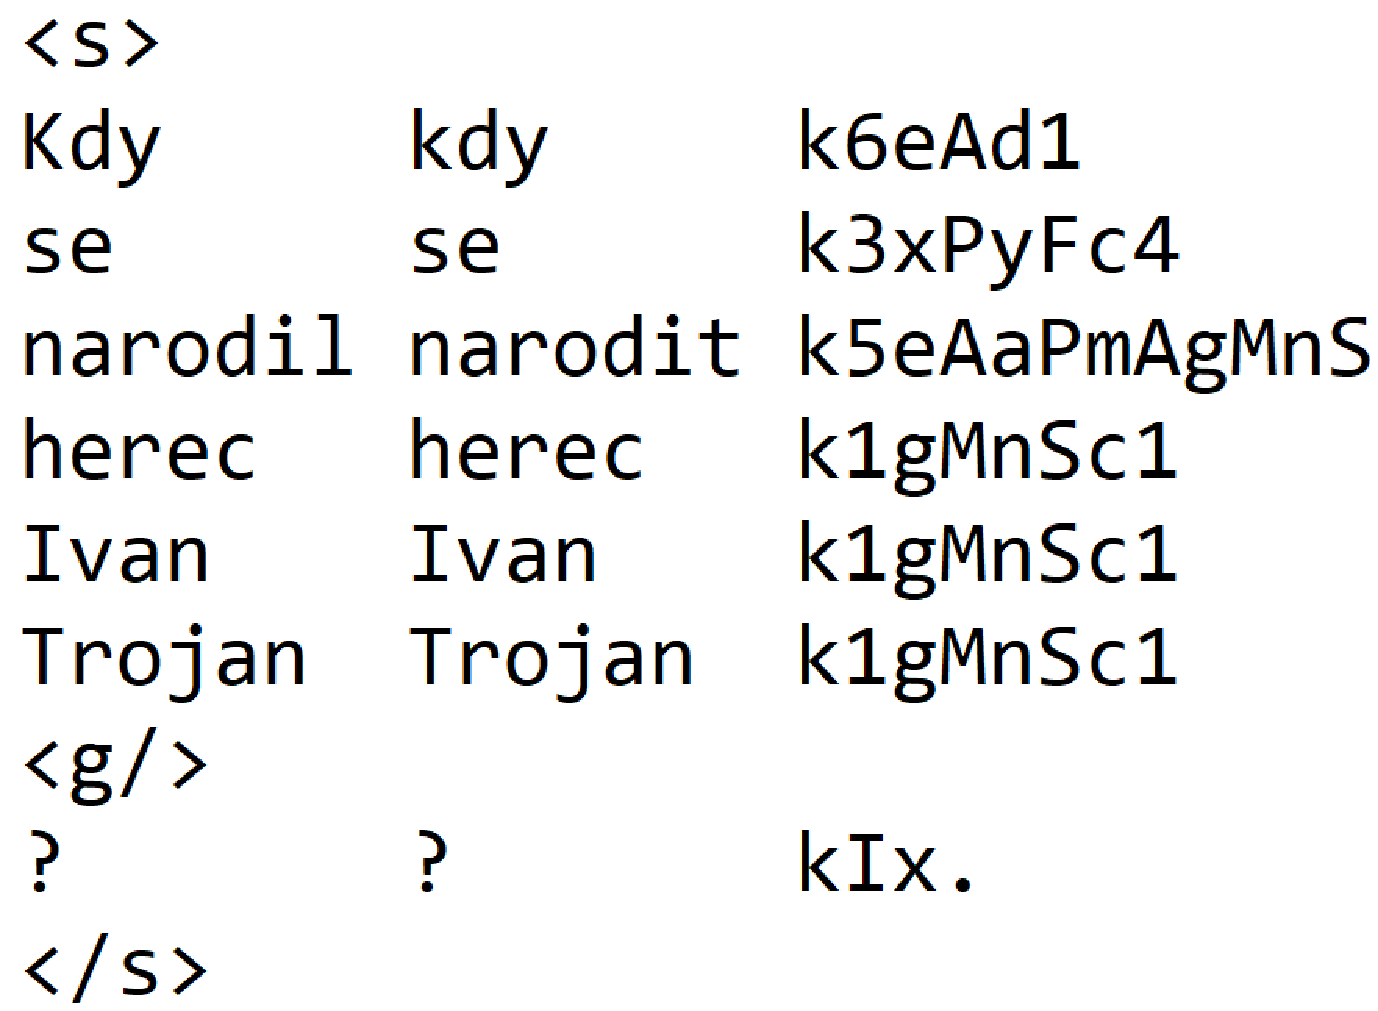
\includegraphics{obrazky/sqad_question_format.pdf}
	}
	\caption{Příklad formátu položky (otázky) datasetu SQAD v3.0.}
	\label{question_format}
\end{figure}

Pro každý záznam musí být tedy otevřeny a~zpracovány soubory obsahující otázku a~odpověď. První sloupec souboru obsahuje na každém řádku \emph{token} otázky, resp. odpovědi, druhý sloupec jejich lemmata. Při zpracování je také potřeba brát ohled na speciální znaky.\par
Pro každý záznam je uložena otázka, extrakce odpovědi a~lemma extrakce odpovědi. Záznamy obsahující ano/ne odpovědi byly ze zpracování vynechány. Zpracovaný dataset je uložen ve formátu JSON (obr. \ref{fig:sqad_processed}) pro jeho pozdější snadnější a~rychlejší použití.

\begin{figure}[hbt]
	\centering
	\scalebox{0.35}{
	    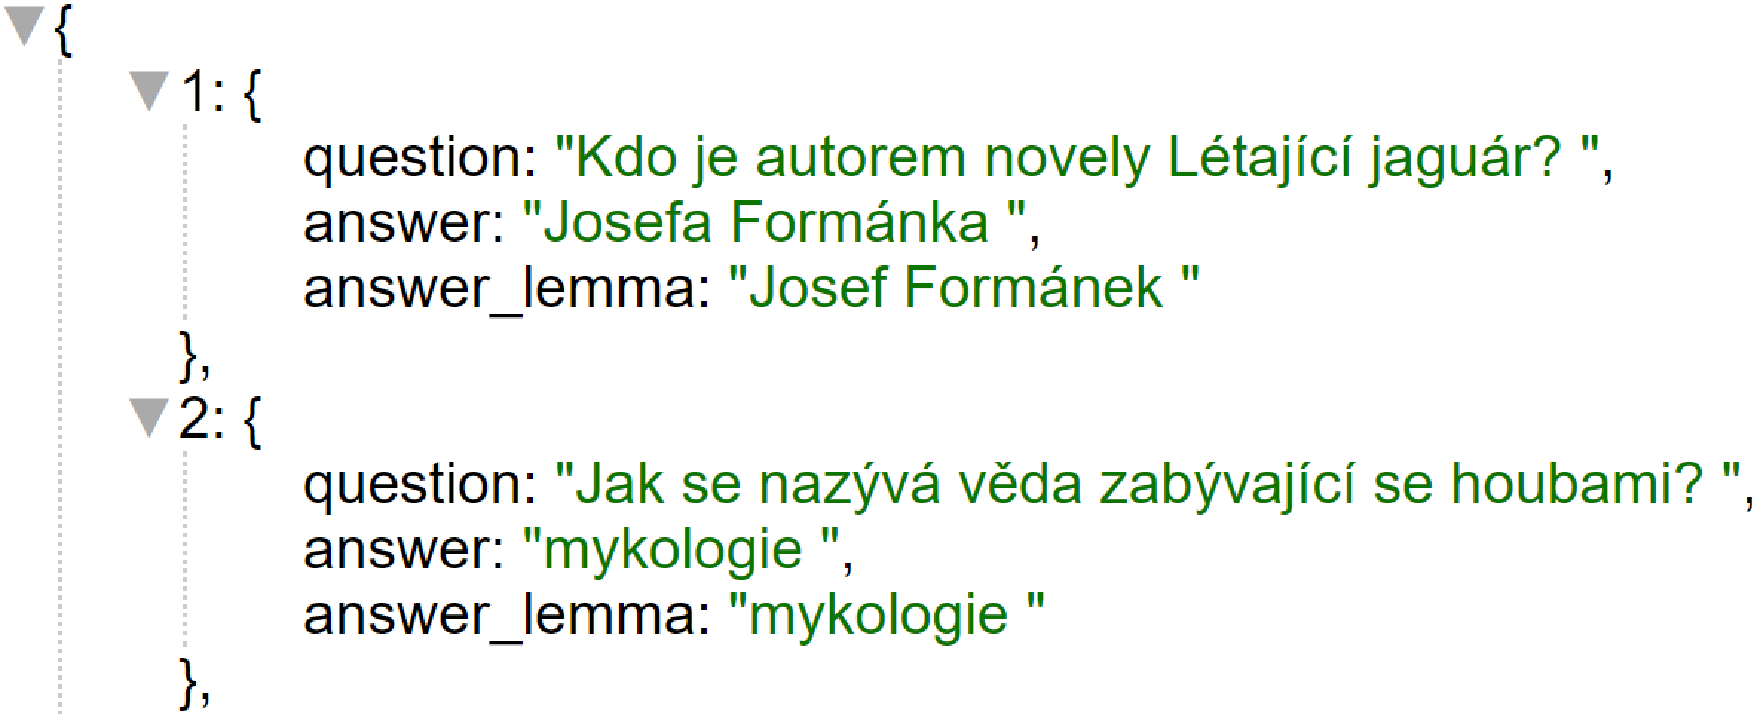
\includegraphics{obrazky/sqad_processed_format.pdf}
	}
	\caption{Příklad formátu zpracovaného datasetu SQAD v3.0.}
	\label{fig:sqad_processed}
\end{figure}
%===========================================================================

\subsection{Ukládání dat pro vyhodnocení systému}
Pro uložení výsledků byl opět zvolen formát JSON, aby mohla být evaluace provedena až po získání odpovědí.\par
\begin{figure}[hbt]
	\centering
	\scalebox{0.52}{
	    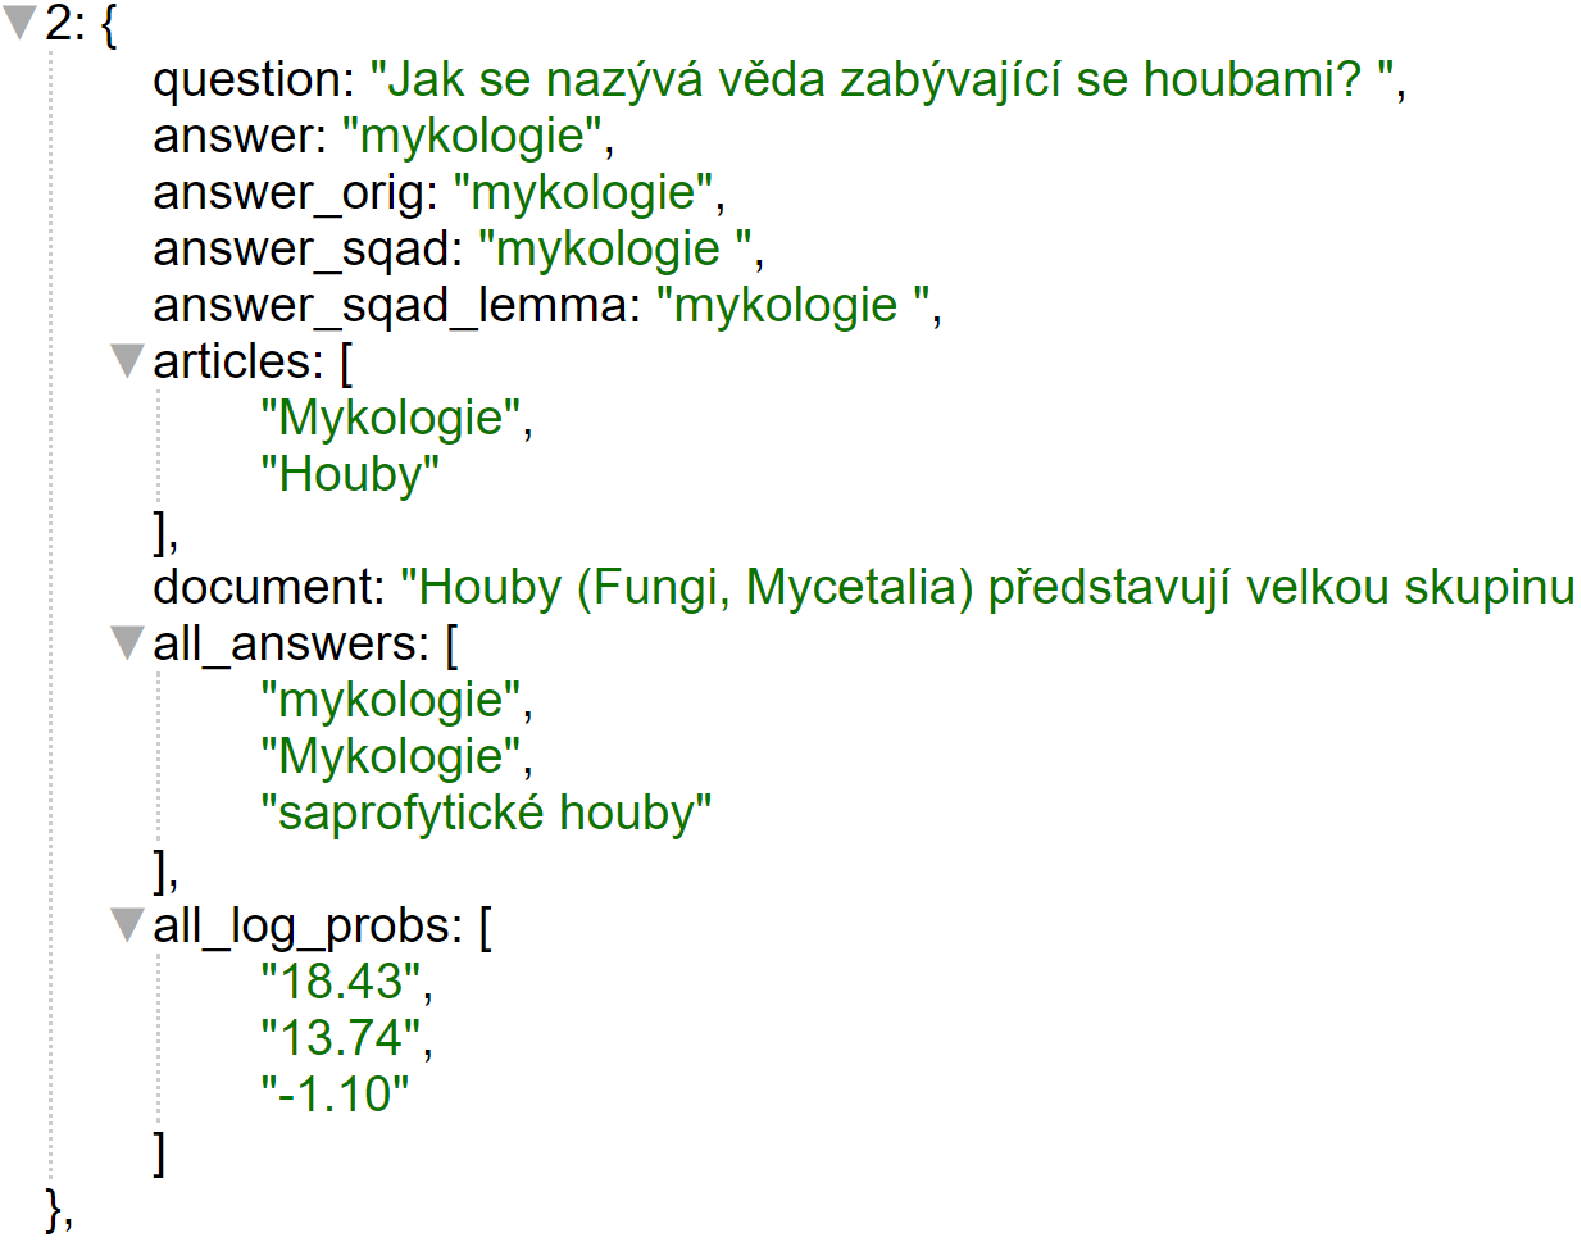
\includegraphics{obrazky/answer_saved_format.pdf}
	}
	\caption{Příklad formátu uložené odpovědi s doplňkovými informacemi.}
	\label{fig:saved_answer}
\end{figure}
Pro každý zodpovězený záznam je uloženo číslo otázky -- \uv{3}, otázka -- \emph{question}, odpověď~--~\emph{answer}, originální/nepřeložená odpověď -- \emph{answer\_orig} (při použití m-BERT readeru shodná s \emph{answer}), referenční odpověď dle datasetu SQAD -- \emph{answer\_sqad} a~její lemma~--~\mbox{\emph{answer\_sqad\_lemma}}. Dále jsou pro podrobnější analýzu výsledků k dispozici názvy článků~--~\emph{articles}, které systém prohledával, kontext -- \emph{document}, ze kterého byla finální odpověď vybrána, první tři nejlepší odpovědi -- \emph{all\_answers} a~skóre -- \emph{scores} jednotlivých odpovědí z \emph{all\_answers}. K dispozici jsou také plné texty nejrelevantnějších pasáží získaných retrieverem -- \emph{all\_documents}.\par
Soubor zodpovězených záznamů je pak pojmenován podle toho, jaký rozsah otázek obsahuje a~přidáno je i časové razítko.
\begin{center}
    answers\_1-3000\_\_04-04-2021\_09:53.json
\end{center}

%=========================================================================
\section{Implementace a~trénink readeru}
\label{reader_imp}
Pro implementaci \emph{readeru} byla použita knihovna\texttt{ transformers }od HuggingFace, která nabízí velmi jednoduché rozhraní pro trénink modelů.\par

\subsection{Trénink}
Pro trénink ALBERT modelu byla použita třída\texttt{ AlbertForQuestionAnswering }a~předtrénovaný model \texttt{albert-base-v2\footnote{\url{https://huggingface.co/albert-base-v2}} }(11 milionů parametrů). Model není příliš velký a~dosahuje podobných výsledků, jako jeho větší verze \texttt{large} nebo \texttt{xlarge}. Pro \emph{fine-tuning} byl použit dataset SQuAD 1.1 a 2.0.\par
Pro druhý model byl použit\texttt{ BertForQuestionAnswering }z knihovny\texttt{ transformers }a předtrénovaný model\texttt{ bert-base-multilingual-cased\footnote{\url{https://huggingface.co/bert-base-multilingual-cased}}} (110 milionů parametrů). Pro fine-tuning byl použit český překlad datasetu SQuAD 1.1 a 2.0. Pro načtení obou datasetů byl použit upravený skript \texttt{squad.py}\footnote{\url{https://github.com/huggingface/datasets/blob/master/datasets/squad/squad.py}} (viz skript \texttt{czech\_squad(2).py}).\par
Všechny modely byly trénovány pomocí třídy\texttt{ Trainer }s následujícími parametry:
\begin{itemize}
    \item \emph{batch size} (velikost dávky) -- $16$
    \item \emph{learning rate} (rychlost učení) -- $2e\!-\!5$
    \item \emph{weight decay} -- $0,01$
    \item \emph{počet trénovacích epoch} -- $3$
\end{itemize}

Po \emph{fine-tuningu} je úspěšnost modelů (F1 a EM, viz \ref{metriky}) na jejich validačních datasetech následující (tabulka \ref{tab:reader_trained}). Oba modely byly trénovány na GPU ve službě Google Colab.

\begin{table}[h]
\centering
    \begin{tabular}{| l | l | l |}
        \hline
        \textbf{ALBERT} & SQuAD 1.1 & SQuAD 2.0 \\ \hline
        EM              & 82,14      & 78,33      \\ \hline
        F1              & 89,58      & 81,55      \\ \hline
    \end{tabular}
    \begin{tabular}{| l | l | l |}
        \hline
        \textbf{mBERT} & cz\_SQuAD 1.1 & cz\_SQuAD 2.0 \\ \hline
        EM              & 68,52      & 66,47      \\ \hline
        F1              & 77,72      & 69,54      \\ \hline
    \end{tabular}
    \caption{
    Úspěšnost modelů na validačních datasetech (v \%).
    }
    \label{tab:reader_trained}
\end{table}

\subsection{Extrakce odpovědi}
Třída zajišťující extrakci odpovědi se nazývá \texttt{Reader} a pro extrakci odpovědi z kontextu je nejprve potřeba vytvořit její instanci. Většina parametrů pro inicializaci je volitelná, musí však být zadána alespoň cesta k natrénovanému modelu v úložišti (\texttt{model\_checkpoint}) a~jeho typ (\texttt{model\_type}). Může být upravena také maximální délka získané odpovědi (pomocí parametru\texttt{ max\_answer\_length}) a max. počet validních odpovědí (\texttt{n\_best\_size}), které model vybere. \emph{Reader} načte tokenizér a model, který bude pro extrakci odpovědi využívat a použije pro jejich akceleraci GPU, pokud je k dispozici.\par
Pro extrakci odpovědi je poté možné volat jedinou instanční metodu \texttt{get\_answers}, která vyžaduje jako parametry otázku a kontext. Vrací pole o velikosti \texttt{n\_best\_size} obsahující nejlepší kandidáty pro odpověď. Každá odpověď se skládá z textu "text"\;a skóre "score".\par
Pro každý dokument je vybrána nejlépe ohodnocená odpověď s neprázdným textem.

%=========================================================================
\section{Implementace retrieveru}
\label{retriever_imp}
Pro získání relevantních dokumentů je implementována třída \texttt{Retriever}. Pro její inicializaci je třeba zadat cestu k modelu pro nástroj MorphoDiTa (\texttt{dita\_file}), který provádí lemmatizaci, cestu k souboru s titulky článků Wikipedie (\texttt{wiki\_titles}) a ke zpracovanému JSON souboru s abstrakty Wikipedie (\texttt{wiki\_abstracts}). Místo MorphoDiTy může \texttt{Retriever} použít i nástroj Majka (\texttt{majka=True}), pro který je potřeba zadat cestu k souboru s morfologickým slovníkem (\texttt{majka\_file}). Pokud není k dispozici zpracovaný soubor s abstrakty, lze původní dump abstraktů převést na formátovaný JSON pomocí funkce \texttt{parse\_abstracts()}.\par
Při vytváření instance \texttt{Readeru} je načten lemmatizátor, sestaven index titulků článků a index abstraktů článků Wikipedie, načten tokenizér (rozdělení na věty) a model pro rozpoznávání entit (pro stažení je třeba nastavit parametr \texttt{download\_ner\_model=True}).\par

\paragraph{Použitá stop slova --}
Pokud je potřeba při zpracování textů v průběhu vyhledávání relevantního dokumentu odstranit stop slova, je pro to využit následující seznam \cite{wiki:frekv}:
\begin{quote}
    {\footnotesize kdy být a se v na ten on že s z který mít do já o k i jeho ale svůj jako za moci pro tak po tento co když všechen už jak aby od nebo říci jeden jen můj jenž ty stát u muset chtít také až než ještě při jít pak před však ani vědět hodně podle další celý jiný mezi dát tady tam kde každý takový protože nic něco ne sám bez či dostat nějaký proto}
\end{quote}
Dále je k dispozici seznam pro odstranění interpunkce:
\begin{quote}
    {\footnotesize . , ? ! ... " ( ) ; - /}
\end{quote}

\paragraph{Tvorba indexu --}
Pro vytvoření indexu pro prohledávání je použita třída \texttt{BM25Okapi} dříve zmíněné knihovny \texttt{rank-bm25}. Každý titulek/abstrakt je převeden na malá písmena, lemmatizován a poté jsou z něj odstraněna stop slova. Získány jsou zpracované tokeny každého titulku/abstraktu. Index titulků/abstraktů je poté vytvořen pomocí \texttt{BM25Okapi} z~takto zpracovaných titulků/abstraktů.

\paragraph{Rozpoznání pojmenovaných entit}(NER - \emph{Named Entity Recognition}) je další úloha na poli NLP. Uveďme alespoň příklad jejího použití:
\begin{center}
    Kdy vynalezl Alfred Nobel dynamit? $\longrightarrow$ Alfred Nobel
\end{center}
NER může usnadnit vyznačení klíčových slov pro vyhledávání.\par
Pro rozpoznání pojmenované entity v otázce je použita knihovna \texttt{deeppavlov}. Využívá natrénovaný model \texttt{ner\_ontonotes\_bert\_mult}, který je načten funkcí \texttt{build\_model()}.

\subsection{Získání relevantních dokumentů}
Inicializace instance třídy \texttt{Retriever} trvá, hlavně kvůli tvorbě indexů a načtení modelu pro NER, poměrně dlouho\footnote{Asi 10 minut, pokud není potřeba stáhnout \texttt{deeppavlov} model pro NER. Pokud lze načíst vytvořený index pomocí modulu\texttt{ pickle}, může to být pouze kolem jedné minuty.}. Po jeho inicializaci je potřeba pro získání relevantních dokumentů pouze jediná instanční metoda \texttt{retrieve()}, která pro zadanou otázku získá $n$ relevantních dokumentů (dle parametru \texttt{max\_docs}).\par
Získání dokumentů probíhá v těle metody \texttt{retrieve()} následovně:
\begin{enumerate}
    \item Nejprve jsou získány názvy článků metodou \texttt{get\_doc\_list()}, které jsou výsledkem vyhledávání metody \texttt{search()} knihovny \texttt{wikipedia}. Jednotlivé vstupy do vyhledávání jsou následující:
    \begin{itemize}
        \item V otázce jsou rozpoznány pojmenované entity (pomocí NER).
        \item Otázka je převedena na malá písmena, lemmatizována a jsou z ní odstraněna stop slova.
        \begin{itemize}
            \item Pomocí metody vytvořeného indexu titulků (\texttt{get\_top\_n()}) je získán nejvíce relevantní titulek článku vzhledem k otázce.
            \item Pomocí metody vytvořeného indexu abstraktů (\texttt{get\_top\_n()}) je získán nejvíce relevantní titulek článku vzhledem k otázce.
        \end{itemize}
        \item Otázka je pro vyhledání použita nezpracovaná.
    \end{itemize}
    Pokud jsou některé výsledky vyhledávání stejné, je použit pouze jeden z nich.
    
    \item Pro každý získaný název článku je získán jeho textový obsah metodou \texttt{page()} kni\-hovny \texttt{wikipedia}. Ten je rozdělen na jednotlivé odstavce a jsou z něj odstraněny nepotřebné části jako reference a odkazy.
    
    \item Je zkontrolováno, jestli některý z odstavců nepřesahuje maximální délku. Je-li potřeba odstavec dále rozdělit, je použita metoda \texttt{normalize\_length()}, která využívá tokenizéru knihovny \texttt{nltk}. Ten rozdělí odstavec na věty, které spojuje, dokud není dosaženo maximální délky pasáže. Pro zbývající věty je vytvořen další odstavec, který obsahuje také poslední 2 věty odstavce předcházejícího.
    
    \item Po normalizaci délky získaných odstavců je potřeba získat jejich zpracovanou verzi, aby mohl být sestaven index pro vyhledávání. Každý odstavec je tedy převeden na malá písmena, lemmatizován a jsou z něj odstraněna stop slova (a interpunkce). Pro každý odstavec je získán seznam takto normalizovaných tokenů, které jsou použity pro tvorbu indexu \texttt{BM25Okapi} pro vyhledávání.
    
    \item Původní lemmatizovaná otázka bez stop slov převedená na malá písmena je použita pro vyhledání v indexu získaných odstavců pomocí metody \texttt{get\_top\_n()}. Tím jsou získány (nezpracované\footnote{Zpracování probíhá pouze pro tvorbu indexu jednotlivých pasáží.}) nejvíce relevantní odstavce -- pasáže pro danou otázku.
\end{enumerate}
\pagebreak
\section*{Nalezení odpovědi na otázku}
Celý tok programu systémem je následující:
\begin{itemize}
    \item Je vytvořena instance třídy pro extrakci odpovědi \texttt{Reader}, instance třídy pro získání relevantních dokumentů \texttt{Retriever} a také instance překladače \texttt{Translator} knihovny \texttt{googletrans} (použití modelu ALBERT).
    
    \item Po zadání otázky je volána funkce \texttt{find\_answer()}, která získá odpověď na otázku.
    \begin{itemize}
        \item Pomocí \emph{retrieveru} jsou získány relevantní dokumenty
        \item V případě použití nativně anglického modelu ALBERT jsou dokumenty spolu s otázkou přeloženy pomocí funkce \texttt{translate()} do angličtiny.
        \item Pro každý získaný dokument je provedena extrakce odpovědi a vybrána nejlépe ohodnocená neprázdná odpověď.
        \item Ze získaných extrakcí odpovědi z jednotlivých dokumentů je vybrána ta, která má nejvyšší skóre. Použita je metoda \texttt{argmax()} knihovny \texttt{numpy}. Pomocí získaného indexu (nejvyšší hodnoty skóre) je vybrán dokument i odpověď.
        \item Vybraná odpověď je při použití modelu ALBERT přeložena zpět do češtiny.
        \item Funkce vrací odpověď. Pro podrobné vyhodnocení dále: dokument, ve kterém byla odpověď nalezena, seznam nejlepších odpovědí, seznam skóre nejlepších odpovědí, seznam článků Wikipedie, které byly pro nalezení odpovědi procházeny a seznam nejlepších pasáží, ze kterých byla provedena extrakce.
    \end{itemize}
\end{itemize}

\section*{Implementace demonstrační aplikace}
Pro předvedení funkčnosti systému byla vytvořena demonstrační aplikace\footnote{Dostupné z adresy \url{http://r2d2.fit.vutbr.cz/.cs}.}, pro kterou byl implementován webový server. Ten je napojen na již dříve existující webový klient. V rámci práce byl tedy pro aplikaci vytvořen pouze backend.

\begin{figure}[hbt]
	\centering
	\scalebox{1}{
	    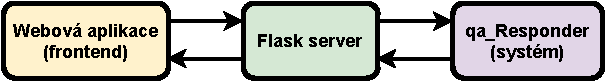
\includegraphics{obrazky/web_demo.pdf}
	}
	\caption{Schéma architektury demonstrační webové aplikace.}
	\label{web_demo_schema}
\end{figure}

Schéma architektury je naznačeno na obrázku \ref{web_demo_schema}. Pro realizaci jednoduchého serveru byl použit framework Flask\footnote{\url{https://flask.palletsprojects.com/}}. Pomocí něj je implementována obsluha několika jednoduchých požadavků, které jsou klientem zasílány.\par

V případě dotazu \texttt{GET} může server poskytnout konfiguraci modelu, výčet předdefinovaných ukázkových otázek a JSON schémata, která určují strukturu konfigurace, požadavku a odpovědi.\par
Při zaslání požadavku \texttt{POST} získá server navíc data ve formátu JSON, která obsahují otázku a požadovanou konfiguraci systému. Server volá pro získání odpovědi metodu\linebreak \texttt{find\_answer() }třídy\texttt{ qa\_Responder}, která zastřešuje systém pro odpovídání.\par
\noindent Metoda získá odpověď na otázku a vrátí ji v určeném formátu. Server poté zašle odpověď ve formátu JSON klientovi, a tím je obsloužen jeho požadavek.\par
\noindent Odpověď serveru ve formátu JSON obsahuje: 
\begin{itemize}
\itemsep-0.1em 
    \item otázku,
    \item jednotlivé odstavce, jejich skóre (získáno hodnotící funkci BM25) a titulek článku každé pasáže,
    \item jednotlivé odpovědi a jejich skóre, pro každou index odstavce, ze kterého pochází a~také index znaku začátku, resp. konce odpovědi (tzv. \texttt{char\_offset}).
\end{itemize}
Maximální počet získaných pasáží a odpovědí je určen konfigurací požadované klientem, která je zaslána jako součást dotazu.
\medskip
\begin{figure}[hbt]
	\centering
	\scalebox{0.8}{
	    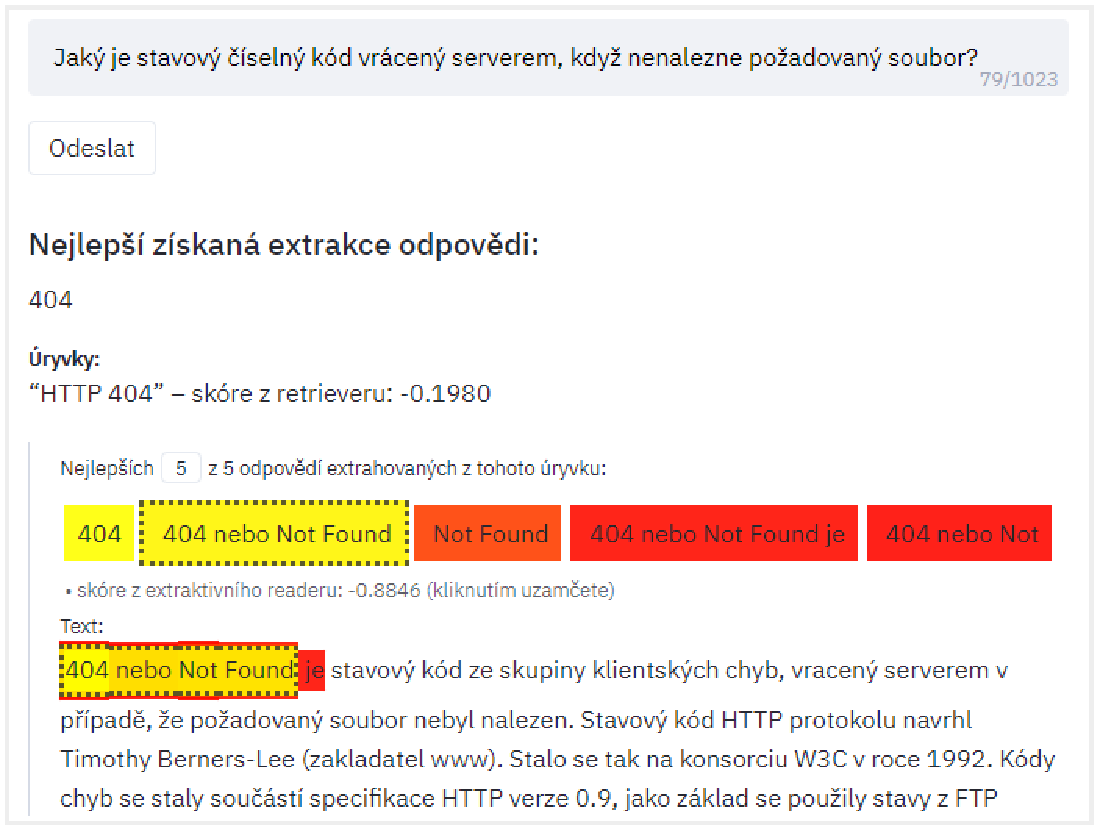
\includegraphics{obrazky/UI.pdf}
	}
	\caption{Příklad použití rozhraní webové aplikace. Na obrázku je vidět otázka, nejlepší nalezená odpověď a jeden ze získaných úryvků textu. U daného úryvku je uveden název článku, ze kterého byl získán, skóre získané retrieverem a nejlepší odpovědi. Pro každou odpověď je uvedeno její skóre dle extraktivního readeru.}
	\label{UI1_example}
\end{figure}

%=========================================================================
%===============================================================================

\chapter{Vyhodnocení systému a~rozbor chyb}
\label{system_evaluation}
V této kapitole jsou popsány výsledky dosažené vytvořeným systémem. Popsán je vliv použitého modelu, trénovacího datasetu a použitého nástroje pro morfologickou analýzu. Nejprve jsou popsány standardní i speciální metriky, na nichž je úspěšnost systému prezentována. Porovnány jsou jednotlivé varianty systému a je provedena i jejich ruční evaluace. Výsledky jsou poté poměřeny s jiným existujícím řešením. Jsou analyzovány chyby a jejich příčiny. Kapitola končí diskuzí o dalším vývoji a vylepšeních.


%=========================================================================
\section{Vysvětlení základních metrik}
\label{metriky}
Tato podkapitola vysvětluje metriky použité pro vyhodnocení systému. Popsány jsou standardní metriky jako EM a F1 používané pro QA systémy a také metriky zachycující specifika otevřené domény.\par
Metody EM a F1 (používané pro vyhodnocení modelů na datasetech SQuAD \cite{squad}\cite{squad_v2}), MRR (např. pro~\cite{sqad}) a částečně T3M jsou standardní metriky používané pro vyhodnocení většiny podobných systémů. Ostatní metriky jsou obměnou těch standardních, navržené specificky pro vyhodnocení tohoto systému.

\subsection{Exact Match (EM)}
\label{EM}
\emph{Exact match}, neboli přesná shoda, je jednoduchá standardní metrika, která ale může diskriminovat dostačující odpovědi s pouze malými rozdíly oproti referenčním výsledkům. Její hodnota může být buď 1 (pokud je shoda dosažena) nebo 0 (pokud se oproti referenční hodnotě výsledek liší, byť jen v jednom znaku). Na příkladu je ukázka penalizace odpovědi, která byla dokonce specifičtější, než referenční odpověď.\par
\begin{center}
\begin{tabular}{l}
    \textbf{otázka:} Kde se narodil Gabriel Jonas Lippmann?\\
    \emph{referenční odpověď:} Bonnevoie\\
    \emph{odpověď systému 1:} Bonnevoie, Lucembursko -- \textbf{EM} = 0\\
    \emph{odpověď systému 2:} Bonnevoie -- \textbf{EM} = 1
\end{tabular}
\end{center}
Při vyhodnocování je referenční i získaná odpověď převedena před porovnáním na malá písmena. Při vyhodnocování varianty systému s modelem ALBERT je brána v úvahu i~původní, nepřeložená odpověď.

\subsection{Exact Lemma Match (ELM)}
\label{ELM}
ELM je speciálně navržená metrika pro toleranci drobných rozdílů oproti referenční odpovědi. Kromě převedení na malá písmena jsou odpovědi před porovnáním také lemmatizovány. Skóre ELM je tedy typicky vyšší, než EM.
\begin{center}
\begin{tabular}{l}
    \textbf{otázka:} Kdy se koná dostihový závod Velká pardubická?\\
    \emph{referenční odpověď:} druhou říjnovou neděli\\
    \emph{odpověď systému:} druhá říjnová neděle \\
    \textbf{EM} = 0 , \textbf{ELM} = 1\\
\end{tabular}
\end{center}

Skóre ELM nabývá opět hodnoty buď 1 (správně) nebo 0 (špatně), stejně jako metrika EM. ELM pro příklad uvedený v \ref{EM} by bylo také 0.

\subsection{Naivní skóre (NS)}
Naivní skóre je nejvíce benevolentní metrikou. Zjišťuje se, zda-li je odpověď, nebo její lemma, podřetězcem referenční odpovědi, nebo jejího lemmatu, případně naopak. Snaha je tedy zachytit co nejvíce alespoň částečně správných odpovědí. Naivní skóre (NS) příkladu uvedeného v podkapitole \ref{EM} a \ref{ELM} je tedy 1. 

\subsection{Top 3 Match (T3M)}
T3M je obdobou EM \ref{EM}, pro shodu je však testována každá z nejlepších třech (3) nalezených odpovědí (případně T\textit{k}M -- nejlepších \textit{k} odpovědí). Můžeme tedy určit, v kolika případech (oproti EM) systém našel správnou odpověď, ale nevybral ji, protože nedosáhla nejvyššího skóre. T3M nabývá opět hodnoty 0, nebo 1.

\subsection{MRR}
MRR (\emph{Mean Reciprocal Rank}) je obdobou T3M, zohledňuje však, na kolikátém místě byla odpověď nalezena (T3M zohledňuje pouze to, jestli vůbec). Pokud má odpověď shodná s~tou referenční nejvyšší skóre (byla vybrána), hodnota MRR je 1, pokud byla na druhém místě, hodnota je 1/2, pokud na třetím, hodnota MRR je 1/3 a tak dále. Pokud nebyla odpověď nalezena vůbec, hodnota MRR je 0 \cite{MRR}.

\subsection{F1 skóre}
Je jakýmsi kompromisem mezi naivním skóre a EM. Při jeho výpočtu jsou použity dvě metriky -- \emph{recall} (úplnost) a \emph{precision} (přesnost) \cite{information_retrieval}.
\begin{equation}
    \text{\textbf{F1}} = 2\cdot \frac{precision \cdot recall}{precision + recall} 
\end{equation}
\begin{equation}
recall = \frac{tp}{tp+fn} \quad precision = \frac{tp}{tp+fp}
\end{equation}

\begin{itemize}
    \item tp -- \emph{true positive} -- znaky (počet) společné pro získanou i referenční odpověď
    \item fn -- \emph{false negative} -- znaky, které jsou v referenční odpovědi, ale chybí v získané
    \item fp -- \emph{false positive} -- znaky, které nejsou v referenční odpovědi, ale přebývají v získané
\end{itemize}

Obvykle jsou definice tp, fn a fp uváděny pro tokeny, ne znaky, chceme ale více zohlednit morfologii češtiny a drobné rozdíly v odpovědích, vztahující se k otevřené doméně. Například augustiánský/augustiánských -- při porovnávání tokenů bychom nedosáhli žádné shody. F1 skóre je počítáno pouze, pokud je získaná odpověď podřetězcem té referenční, nebo naopak.\par \medskip
\noindent Pro příklad: 
\begin{center}
\begin{tabular}{l}
    \textbf{otázka:} Odkud byla anglická kapela The Beatles?\\
    \emph{referenční odpověď:} z Liverpoolu\\
    \emph{odpověď systému:} Liverpoolu\\
\end{tabular}
\end{center}
je tedy $precision = 1$, $recall = 0,83$ a $\text{\textbf{F1}} = 0,91$.\par \medskip
\noindent Pro příklad z \ref{EM}
\begin{center}
\begin{tabular}{l}
    \textbf{otázka:} Kde se narodil Gabriel Jonas Lippmann?\\
    \emph{referenční odpověď:} Bonnevoie\\
    \emph{odpověď systému:} Bonnevoie, Lucembursko\\
\end{tabular}
\end{center}
je $precision = 0,41$, $recall = 1$ a $\text{\textbf{F1}} = 0,82$.\par \medskip
F1 tedy zohledňuje přesnost i úplnost odpovědi a je velmi směrodatnou metrikou při odpovídání na otázky.

\subsection{Lidské vyhodnocení}
Otevřená doména je problematická pro automatické vyhodnocování. Jak je uvedeno například v \cite{min2021neurips}, otázka může mít více možných odpovědí, pokud není jednoznačně položena. Odpověď může být také obecnější, nebo specifičtější (př. z \ref{EM}), ale stále odpovídat na otázku. Z článku \cite{min2021neurips} tedy vyplývá, že systémy jsou hodnoceny lépe při vyhodnocení lidmi. Konkrétně, procento odpovědí označených jako \uv{rozhodně správně} bylo u systémů v průměru o 17--25 \% lepší, než pouhé porovnání řetězců odpovědí pomocí EM.\par
Proto je náhodně vybráno 200 otázek pro lidské vyhodnocení každé varianty systému, aby se bral alespoň minimální ohled na diskriminační povahu automatické evaluace.

%=========================================================================
\section{Vyhodnocení výsledného open-domain systému}
Pro vyhodnocení celého systému byla vybrána datová sada SQAD v3.0 \cite{sqad}, ze které byly odebrány ano/ne otázky.\par
Pro každou metriku z podkapitoly \ref{metriky} bylo použito vzorce \ref{score_calc},
\begin{equation}
    \label{score_calc}
    \text{skóre} = \frac{1}{N}\cdot \sum^N_{k=1} S_k
\end{equation}
kde $S_k$ je skóre $S$ (např. EM) pro odpověď $k$ a $N$ je celkový počet odpovědí. Skóre na celém datasetu je tedy průměrem jednotlivých skóre $S_k$ všech zodpovězených otázek.\par
V této podkapitole jsou shrnuty a porovnány výsledky systému na testovací sadě. Pro každou variantu systému bylo provedeno vyhodnocení pouze na (stejné) čtvrtině\footnote{Velikost čtvrtiny datasetu je \textbf{2819 vzorků} -- srovnatelné s počtem vzorků při vyhodnocení AQA v \cite{aqa2018}.} datasetu, která byla získána vybráním každého čtvrtého vzorku. Pro vítěznou variantu bylo vyhodnocení provedeno na všech (více jak 11\,000) otázkách.

\subsection{Model ALBERT a strojový překlad}
\label{albert_eval}
Tato část prezentuje vyhodnocení systému s readerem ALBERT, pro který jsou získané pasáže a otázka strojově překládány do angličtiny. Vyhodnocení proběhlo pro 4 varianty: porovnán byl trénovací dataset -- SQuAD 1.1/2.0 (SQ1.1/2.0) a nástroj použitý pro morfologickou analýzu -- Majka/MorphoDiTa (Maj/MD). Nejlepší výsledky a důležité metriky, jako EM a F1, jsou zvýrazněny tučně.

\begin{table}[H]
    \centering
    \begin{tabular}{|l||l|l|l|l|l|l|l|l|l|}
        \hline
        \textbf{ALBERT}  & \textbf{EM}   & ELM       & NS        & T3M       & MRR       & \textbf{F1}   & prec.         & rec. \\ \hline\hline
            SQ1.1+MD    & 11,96         & 25,63     & 37,77     & 23,61     & 21,17     & 22,93         & 21,80         & 25,81    \\ \hline
            SQ2.0+MD    & 12,85         & 26,08     & 39,57     & 23,63     & 21,66     & 23,87         & 22,77         & 26,80    \\ \hline
            SQ1.1+Maj   & 11,64         & 25,37     & 37,90     & \textbf{23,78}     & 21,40     & 23,03         & 21,88         & 25,98    \\ \hline
            SQ2.0+Maj   & \textbf{12,88}& \textbf{26,15}& \textbf{39,60}& 23,60     & \textbf{21,68}     & \textbf{24,11}         & \textbf{22,98}         & \textbf{27,09}    \\ \hline
    \end{tabular}
    \caption{Úspěšnost systému [\%] s readerem ALBERT a strojovým překladem textů -- vyhodnoceno pro čtvrtinu datasetu SQAD v3.0 (2819 otázek).}
    \label{tab:system_eval_albert}
\end{table}
Jak je vidět v tabulce \ref{tab:system_eval_albert}, výsledky tohoto přístupu nejsou příliš dobré. Za povšimnutí stojí výrazný rozdíl mezi EM a ELM. Příčinou tak velké odchylky od přesné shody je nejspíš ztráta původního tvaru slov/frází při překladu, kdy však slovní základ zůstává stejný. Naivní skóre dosahuje téměř 40 \%, nějaké shody tedy systém dosáhl, ale nepřesnosti způsobené překladem převládají.

\subsection{Model vícejazyčný BERT}
\label{mbert_eval}
Vyhodnocení systému, používajícího vícejazyčný BERT jako reader, proběhlo opět ve 4 variantách, stejně jako v předchozí podkapitole \ref{albert_eval}. Značení je stejné s jediným rozdílem, kdy SQ1.1/2.0 jsou českými strojovými překlady datové sady SQuAD použité pro trénink readeru. Nejlepší výsledky jsou opět zvýrazněny tučně.

\begin{table}[H]
    \centering
    \begin{tabular}{|l||l|l|l|l|l|l|l|l|l|}
        \hline
        \textbf{mBERT}  & \textbf{EM}   & ELM       & NS        & T3M       & MRR       & \textbf{F1}   & prec.         & rec.      \\ \hline\hline
            SQ1.1+MD    & 41,22         & 43,17     & 59,67     & 46,68     & 43,73     & 52,31         & 54,77         & 53,07     \\ \hline
            SQ2.0+MD    & \textbf{42,85}&\textbf{44,84}&\textbf{61,83}&\textbf{47,11}&\textbf{44,80}&\textbf{54,33}&\textbf{56,94}&\textbf{55,04}\\ \hline
            SQ1.1+Maj   & 40,90         & 42,85     & 59,13     & 46,29     & 43,38     & 51,79         & 54,27         & 52,55         \\ \hline
            SQ2.0+Maj   & 42,36         & 44,38     & 61,16     & 46,65     & 44,32     & 53,63         & 56,26         & 54,35     \\ \hline
    \end{tabular}
    \caption{Úspěšnost [\%] systému s readerem m-BERT trénovaném na českém překladu datasetu SQuAD -- vyhodnoceno pro čtvrtinu datasetu SQAD v3.0 (2819 otázek).}
    \label{tab:system_eval_mbert}
\end{table}

Při použití vícejazyčného modelu BERT bylo dosaženo lepších výsledků (tab. \ref{tab:system_eval_mbert}) a jeho nejlepší varianta je tedy dále vyhodnocena na všech 11\,273 otázkách testovací datové sady.\par
Následuje ještě ale podkapitola o ručním vyhodnocení lidmi, která zachycuje diskriminační povahu automatických metrik a lépe charakterizuje použitelnost systému.\pagebreak

\subsection{Vyhodnocení člověkem}
\label{human_eval}
Z celé datové sady SQAD v3.0 bylo náhodně vybráno 200 otázek, které byly vyhodnoceny také ručně -- lidmi (inspirováno \cite{min2021neurips}). Porovnána na nich je úspěšnost jednotlivých systémů dle automatického vyhodnocení\footnote{U tohoto vzorku a lidských hodnotitelů jsou pro porovnání vybrány pouze metriky EM a F1.} a vyhodnocení lidmi. Je tedy zjišťováno, zda by danou odpověď systému bral člověk jako postačující.\par
Následující tabulka \ref{tab:human_eval} prezentuje přehledně zjištěné hodnoty.

\begin{table}[H]
\centering
\begin{tabular}{|l||l|l|l|}
    \hline
        {ALBERT}       & \textbf{EM} & \textbf{F1} & \textbf{člověk} \\ \hline\hline
    SQ1.1+MD  & 11,00       & 24,46       & 55,50               \\ \hline
    SQ2.0+MD  & 11,00       & 24,48       & 54,50               \\ \hline
    SQ1.1+Maj & 11,00       & 24,48      & \textbf{56,50}               \\ \hline
    SQ2.0+Maj & \textbf{12,00}       & \textbf{24,92}      & 53,50               \\ \hline
    \end{tabular}
    \begin{tabular}{|l||l|l|l|}
    \hline
    {mBERT}       & \textbf{EM} & \textbf{F1} & \textbf{člověk} \\ \hline\hline
    SQ1.1+MD  & 43,00       & 53,15         & 64,00               \\ \hline
    SQ2.0+MD  & \textbf{46,00}& \textbf{56,81}& \textbf{69,00}              \\ \hline
    SQ1.1+Maj & 42,00       & 52,55           & 63,00               \\ \hline
    SQ2.0+Maj & 45,00       & 56,21           & 67,50               \\ \hline
    \end{tabular}
\caption{Porovnání automatického a ručního vyhodnocení variant systémů vyhodnocených v \ref{albert_eval} a \ref{mbert_eval} na 200 náhodně vybraných otázkách.}
\label{tab:human_eval}
\end{table}

Pro metriku \uv{člověk} byla odpověď ohodnocena 1, pokud byla při ručním vyhodnocení posouzena jako dostačující. U výsledků je vidět rozdíl mezi EM a lidským vyhodnocením až 45,5 \% (pro systém využívající strojový překlad a reader ALBERT). Až 23 \% pak pro systém využívající vícejazyčný BERT.\par
Výsledky tedy indikují použitelnost odpovědi až v 70 \% případů (pro nejlepší variantu systému). Také ukazují mnohem vyšší použitelnost výsledků prvního přístupu (reader ALBERT), než se při automatickém vyhodnocení mohlo zdát. Nedosahují však kvalit systému využívajícího vícejazyčný BERT.\par
Pro ilustraci je uvedeno pár příkladů, které byly při ručním vyhodnocení posouzeny jako dostačující:

\begin{table}[H]
\centering
\begin{tabular}{|l|l|}
\hline
\textbf{č.}   &\textbf{Otázka}                                         \\ \hline
1               &Kolik má čeština slovních druhů?                        \\ \hline
2                &Kdo je Oldřich Homuta?                                  \\ \hline
3                &Která diecéze má jako hlavní patronku svatou Zdislavu?  \\ \hline
4                &Jaké je jméno současného papeže?                        \\ \hline
5                &Kdo je vrchním velitelem ozbrojených sil ČR?            \\ \hline
6                & Kde zemřel Platón?                                      \\ \hline
\end{tabular}
\begin{tabular}{|l|l|l|}
\hline
\textbf{č.}   &\textbf{Odpověď systému} & \textbf{Referenční odpověď} \\ \hline
1               &deset                    & 10                          \\ \hline
2               &český elektrotechnik     & vynálezce remosky           \\ \hline
3               &litoměřické diecéze      & litoměřický                 \\ \hline
4               &kardinál Bergoglio       & František                   \\ \hline
5               &Miloš Zeman              & prezident České republiky   \\ \hline
6               &Atény                    & v Athénách                  \\ \hline
\end{tabular}
\caption{Příklady odpovědí systému (různých variant z vyhodnocovaných), které byly posouzeny člověkem jako dostačující.}
\label{tab:human_eval_examples}
\end{table}

\subsection{Porovnání dosažených výsledků}
Vyhodnocení jednotlivých variant systému proběhlo v předchozích podkapitolách, a mohou být tedy shrnuty závěry experimentů. \par
Pro variantu ALBERT došlo oproti variantě mBERT pouze k velmi malé přesné shodě získaných výsledků. Pro obě varianty systému byl úspěšnější \emph{reader} trénovaný na verzi 2.0 datasetu SQuAD, tedy na tom, který pro trénink obsahuje i velké množství dokumentů neobsahujících odpověď na položenou otázku. Tento trénink nejspíš přispěl k častějšímu výběru správného dokumentu.\par
Co se týká lexikálních analyzátorů a jejich vlivu na funkci hodnotící funkce \texttt{bm25}, zvítězil v první variantě analyzátor Majka, ne však příliš přesvědčivě a procentuální rozdíl oproti MorphoDiTě je téměř zanedbatelný. Pro druhou variantu zvítězil analyzátor MorphoDiTa, a to o něco přesvědčivěji. Ve všech experimentech byl však rozdíl v systémech používajících různý lexikální analyzátor velmi malý. Kvůli tomu, že byl však ve druhé (úspěšnější) variantě nástroj MorphoDiTa systematicky (byť jen o trochu) lepší, je použit pro vyhodnocení systému na celé testovací datové sadě právě on.\par
Co se týká ručního vyhodnocení lidmi, byly všechny varianty mnohem úspěšnější, než podle automatického vyhodnocení. Větší rozdíl mezi automatickým a lidským vyhodnocení byl zaznamenán u první varianty systému s readerem ALBERT, kde jsou fráze deformovány opakovaným překladem textu do angličtiny a zpět do češtiny. Reálná použitelnost této varianty systému však není tak špatná, jak se z automatického vyhodnocení zdá.\par
Z provedených experimentů je tedy vítěznou variantou systém mBERT SQ2.0+MD. Tedy systém používající jako reader vícejazyčný BERT natrénovaný na českém překladu datasetu SQuAD 2.0 a nástrojem MorphoDiTa pro morfologickou analýzu.

\subsection{Vyhodnocení nejlepšího dosaženého systému}
\label{best_eval}
V této části jsou uvedeny výsledky vyhodnocení nejlepší varianty systému na celém datasetu SQAD 3.0. Experimentováno bylo s množstvím dokumentů, které jsou předány readeru k~extrakci odpovědi. V tabulce \ref{tab:final_evaluation} jsou uvedeny výsledky vyhodnocení systému.
\begin{table}[H]
    \centering
    \begin{tabular}{|l||l|l|l|l|l|l|l|l|l|}
        \hline
          & \textbf{EM}   & ELM       & NS        & TkM       & MRR       & \textbf{F1}   & prec.         & rec. \\ \hline\hline
            top 3    & 42,30         & 44,21     & 61,20     & 46,67     & 44,27     & 53,69         & 56,12         & 54,44    \\ \hline
            top 5    & 43,71         & 45,64     & 62,80     & 50,02     & 46,41     & 55,20         & 57,62         & 55,95    \\ \hline
            top 8   & \textbf{43,89}         & \textbf{45,83}     & \textbf{62,96}     & 52,36     & 47,34     & \textbf{55,42}         & \textbf{57,70}         & \textbf{56,28}    \\ \hline
            top 10   & 43,77         & 45,68     & 62,87     & \textbf{53,07}     & \textbf{47,48}     & 55,28         & 57,52        & 56,17    \\ \hline
    \end{tabular}
    \caption{Vyhodnocení systému [\%] na celém datasetu SQAD 3.0 (bez ano/ne otázek --~viz tabulka \ref{tab:sqad_size}) s~využitím Wikipedie jako báze znalostí. Porovnáno je množství čtených dokumentů \uv{top~\emph{k}}. TkM je varianta metriky T3M (\ref{metriky}) pro různý počet top \emph{k} čtených dokumentů. Varianta systému: extraktivní reader -- vícejazyčný BERT trénován na datasetu cz\_SQuAD 2.0 (\ref{reader_imp}), morfologický analyzátor -- MorphoDiTa.}
    \label{tab:final_evaluation}
\end{table}
Při vyhodnocení na celé testovací sadě se hodnoty od výsledků na čtvrtině datasetu v~podkapitole \ref{mbert_eval} o mnoho neliší. Z tabulky \ref{tab:final_evaluation} vyplývá, že nejlepší pro maximalizaci skóre EM i většiny dalších je čtení 8 nejvíce relevantních dokumentů. Při hodnotě 10 už úspěšnost většiny metrik klesla. Zvýšilo se však skóre TkM i MRR, což je s větším množstvím získaných dokumentů očekávatelné.

%=========================================================================
\section*{Porovnání výsledků práce se současným stavem poznání}
V této podkapitole jsou výsledky práce porovnány s podobnými systémy stejného účelu, pro které je dostupné vyhodnocení na standardních metrikách.\par
\begin{table}[H]
\centering
\begin{tabular}{|l|l|c||l|l|}
\hline
systém     & dataset   & počet testovacích otázek & \textbf{EM} & \textbf{NS} \\ \hline \hline
AQA 2018   & SQAD v1.0 & 3 301                    & 49,83       & 59.58       \\ \hline
AQA 2018   & SQAD v1.1 & 3 301                    & 38,08       & 46,26       \\ \hline
\textbf{Tato práce} & SQAD v3.0 & 11 273                   & 43,89       & 62,96       \\ \hline
\end{tabular}
\caption{Porovnání výsledků této práce se systémem AQA \cite{aqa} (uvedené výsledky jsou převzaty z \cite{aqa2018}). Výsledky jsou uvedeny v \%.}
\label{tab:aqa_compare}
\end{table}
Výsledky práce jsou porovnány s výsledky systému AQA \cite{aqa}, konkrétně s poslední dostupnou vyhodnocenou variantou tohoto systému z roku 2018 \cite{aqa2018}, která byla vyhodnocena na 3301 otázkách z datasetu SQAD v1.0 a 1.1. Výsledky jsou shrnuty v tabulce \ref{tab:aqa_compare} a jsou porovnány pomocí metrik EM a NS. Metrika NS není v práci specifikována, pracuje se v~ní však s \uv{plnou shodou} (EM) a \uv{částečnou shodou}, která je definována jako odpověď, která se přesně neshoduje s referenční, protože některá slova přebývají, nebo chybí. \emph{Částečná shoda} uváděna při vyhodnocení systému AQA je tedy značena jako NS -- naivní skóre (viz~\ref{metriky}), což je metrika této práce, která popisu nejvíce odpovídá. NS pro AQA je součtem hodnot \emph{plné} a \emph{částečné} shody (uvedených v \cite{aqa2018}).\par
Z výsledků uvedených v tabulce \ref{tab:aqa_compare} je patrné, že systém AQA převyšuje výsledky této práce pouze v metrice EM, a to pouze na části zastaralého datasetu SQAD v1.0. Z tabulky je patrné (a je tak uvedeno i v práci \cite{aqa2018}), že při vyhodnocení na stejně velkém vzorku vybraného z aktualizované verze datasetu 1.1 úspěšnost systému výrazně klesla (z EM 49,83~\% na EM 38,08 \%). Takový (možná i výraznější) pokles by šlo očekávat i při vyhodnocení systému na datasetu SQAD v3.0 použitého v této práci -- ta navíc vyhodnocuje systém na výrazně větším počtu vzorků. Systém prezentovaný v mé práci navíc dosahuje výrazně vyšších hodnot naivního skóre, které koresponduje s procentem použitelných výsledků více, než přesná shoda (jak je uvedeno v části \ref{human_eval}).\par
Výsledky práce tedy považuji v porovnání s dostupným vyhodnocením systému AQA, který představuje relevantní porovnání s výsledky mé práce, za úspěch.\par
Výsledky mohou být porovnány také se \textit{state of the art} systémy, které však existují pouze pro angličtinu a jsou vyhodnoceny na datasetu NQ. Například v podkapitole \ref{existing_work} zmíněný systém R2-D2 (55 \% EM), nebo nejlepší výsledky na datasetu NQ uvedené v jeho oficiálním žebříčku (až 64 \% F1). Rozdílnost datasetu (a jazyku) sice neposkytuje příliš validní porovnání, jsem ale přesvědčen, že výsledky této práce takových kvalit nedosahují. Přesto si systém v porovnání s existujícími systémy nevede špatně.


%=========================================================================
\section{Rozbor chyb a~možnosti dalšího vývoje}
V této podkapitole jsou rozebrány nedostatky systému, příčiny nesprávných odpovědí a možnosti vylepšení/nahrazení jeho existujících komponent pro jeho optimálnější funkci.\par
\subsection{Analýza chyb a jejich příčin}
Dataset je pro analýzu chyb nejprve rozdělen na 5 částí, které byly vyhodnoceny samostatně. Z každé části jsou uloženy nesprávné odpovědi. Ty jsou blíže zkoumány pro část testovacích vzorků s nejnižší úspěšností. Úspěšnost na jednotlivých částech je uvedena v tabulce \ref{tab:partial_eval}.

\begin{table}[H]
\centering
\begin{tabular}{|l|l|l|l|l|}
\hline
           & \textbf{EM} & \textbf{F1} & \textbf{NS} & \textbf{MRR} \\ \hline
\textbf{1} & 57,69       & 65,70       & 71,26       & 60,89        \\ \hline
\textbf{2} & 40,75       & \textbf{52,09}       & 59,69       & 44,61        \\ \hline
\textbf{3} & 41,65       & 53,57       & 61,54       & 44,89        \\ \hline
\textbf{4} & \textbf{38,70}       & 53,36       & 62,19       & \textbf{42,16}        \\ \hline
\textbf{5} & 40,68       & 52,38       & \textbf{60,07}       & 44,18        \\ \hline
\end{tabular}
\caption{Vyhodnocení systému na jednotlivých pětinách datasetu (1--5), kde každá pětina má asi 2255 vzorků. Pro první pětinu jsou tedy vyhodnoceny vzorky s číslem 1 až 2255. Tučně jsou uvedeny nejnižší hodnoty (v \%).}
\label{tab:partial_eval}
\end{table}

Nejlépe dopadla při vyhodnocení s velkým náskokem první část vyhodnocovací sady. Nejhůře část 4 (otázky 6765--9020), kde přesná shoda nedosáhla 40 \%. Pro tuto část je tedy proveden rozbor chyb. Pro rozbor byly vybrány vzorky, u kterých nebylo dosaženo přesné shody, nebo bylo dosažené F1 skóre menší než 0,5. Získáno tak bylo 982 vzorků pro bližší analýzu.\par
Prvním směrodatným údajem je skóre TkM -- tedy přesná shoda v alespoň jedné extrakci odpovědi, která byla pro přečtené dokumenty provedena. Hodnota tohoto skóre dosahuje 15,78 \%. Tyto chyby jsou tedy způsobeny špatným výběrem získané odpovědi, která je závislá na skóre určeném \emph{readerem}.\par
Ze zbývajících 827 vzorků bylo dosaženo NS 13,66 \%, což indikuje alespoň minimální použitelnost tohoto zlomku získaných odpovědí. Zbývá tedy zjistit příčinu chyb u 714 odpovědí, kde nebylo dosaženo žádné shody.\par
Pro zbývající vzorky bylo provedeno vyhodnocení, které má za úkol zjistit, jestli se referenční odpověď nachází v některém z top $n$ (pro analyzovaný systém $n=8$) dokumentů. Ta byla nalezena ve 37,11 \% analyzovaných vzorků. Pro tyto shody bylo vypočítáno také skóre MRR 25,68 \%, které zhodnocuje i pořadí relevance těchto dokumentů, ve kterém byly získány retrieverem.\par
Z původních 982 analyzovaných chybných vzorků můžeme tedy 533 považovat za chybnou extrakci odpovědi, nebo její špatné ohodnocení a vybrání nesprávné. Pro zbylých 449 vzorků nebyla správná odpověď nalezena v jediném získaném dokumentu. Vzhledem k původnímu vzorku pětiny datasetu (2255 zodpovězených otázek) je to tedy asi 20 \%. Výsledky této analýzy prezentuje tabulka \ref{tab:error_analysis}.

\begin{table}[H]
\centering
\begin{tabular}{|l||c|c|c|}
\hline
\textbf{typ chyby}                & \multicolumn{1}{l|}{\textbf{zastoupení (v \%)}} & \multicolumn{1}{l|}{\textbf{počet}} & \multicolumn{1}{l|}{\textbf{původ chyby}}                                              \\ \hline
nevybrání správné odpovědi        & 15,78                                          & 155                                              & \multirow{3}{*}{reader (54 \%)}                                                       \\ \cline{1-3}
nízká shoda s referenční odpovědí & 11,51                                          & 113                                              &                                                                                        \\ \cline{1-3}
chybná extrakce (nulová shoda)    & 26,99                                          & 265                                              &                                                                                        \\ \hline
nenalezení relevantního dokumentu & 35,95                                          & 353                                              & \multirow{2}{*}{\begin{tabular}[c]{@{}c@{}}retriever /\\ auto. vyhod.\end{tabular}} \\ \cline{1-3}
správná odpověď (ručně)           & 9,77                                           & 96                                               &                                                                                        \\ \hline
\end{tabular}
\caption{Příčiny chyb v analyzovaném vzorku 982 chybně zodpovězených otázek.}
\label{tab:error_analysis}
\end{table}

Pro otázky, které nebyly správně zodpovězeny a byly klasifikovány jako chyba retrieveru, protože nedošlo k nalezení relevantního dokumentu obsahujícího referenční odpověď, bylo provedeno ruční vyhodnocení. V těchto 449 otázkách bylo nalezeno 96 odpovědí, které jsou při ručním vyhodnocení člověkem postačující. Zbylo tedy 353 vzorků a z ručního vyhodnocení vyplývá několik hlavních příčin chyb:
\begin{itemize}
    \item mnohoznačnost otázky/otázka nedává bez kontextu smysl,
    \begin{itemize}
        \item \uv{Proč se Severu nedostávalo zkušených vojevůdců?}, \uv{Proč Franco zaútočil na severu?}, \uv{Co udělal Smith v roce 1999?}, \dots
    \end{itemize}
    \item správná odpověď se nachází mezi nevybranými, je však v jiném tvaru,
    \item po převodu na malá písmena (viz \ref{retriever_imp}) se ztrácí část kontextu,
    \item nebyly získány dostatečně relevantní dokumenty,
    \item neschopnost readeru identifikovat ve složitém kontextu odpověď -- je také možné, že byla nalezena, neměla však nejvyšší skóre v dané pasáži.
\end{itemize}

\subsection{Další vývoj a možnosti navazujících prací}
Práce pokládá základ systému, který nabízí velký prostor pro další vylepšení. Návrhy toho, jak by mohlo být řešení rozšířeno například v rámci navazujících prací je popsáno v této části.\par
Nejdříve, co se týká první části systému -- retrieveru pro získávání relevantních pasáží. Řazení pomocí hodnotící funkce BM25 by mohlo být nahrazeno modernějším přístupem DPR popisovaným v části \ref{dpr}, ať už za použití vícejazyčného modelu BERT, nebo jiného modelu (enkodéru) pro získání vektorové reprezentace. Pro získávání pasáží by oproti přístupu v~této práci, kdy jsou procházeny pouze relevantní články, mohla být vhodně zpracována a~indexována celá Wikipedie, případně by mohly být zpracovány i zvláštní struktury, jako tabulky, kde se často nachází spousta relevantních informací. Při zpracování textu by mohl být vylepšen také převod na malá písmena, aby nedocházelo ke ztrátám kontextu.\par
Co se týká modulu pro extrakci odpovědi, jsou cesty dalšího vývoje velmi otevřené. Prvním vylepšením by mohl být modul pro odhad předmětu otázky, aby došlo k lepší shodě při výběru odpovědi (otázka se ptá na datum -- uvažujme pouze odpovědi, které jsou také datum). Zajímavé by mohlo být také experimentovat s další variantou modelu BERT použitelného pro češtinu -- například Slavic BERT \cite{slavicBERT}. Mimo existující předtrénované enkodéry by měl být předmětem výzkumu hlavně předtrénink ryze české varianty (například modelu ALBERT). Takový pokus již sice byl uskutečněn (práce \cite{Zelina2020thesis}), model však nedosahoval dostatečných kvalit. Dále by se dalo experimentovat s přidáním generativního (abstraktivního) readeru, jak je učiněno například v \cite{fajcik2021pruning} (systém R2-D2).\par
Zajímavá by mohla být práce s datasetem COSTRA \cite{costra}, který se zaměřuje na embedding na úrovni vět, konkrétně pochopení jejich významu bez ohledu na drobné rozdíly v~jejich formulaci. Modifikace, na které se dataset zaměřuje, jsou různé druhy parafrází, generalizace, konkretizace, převrácení významu a další. Dataset původně vznikl pro češtinu a~mohl by pomoct k jejímu lepšímu pochopení modelem.\par
Přínosné by bylo také další rozšíření datasetu SQAD nebo tvorba nového datasetu zaměřeného na otevřenou doménu, obsahující více reálných příkladů toho, na co se lidé ptají na internetu -- ať už pro účel tréninku retrieveru (DPR), nebo pro reálnější vyhodnocení schopností takového systému.

%=========================================================================
%===============================================================================

\chapter{Závěr}
\label{conclusion}
Práce se zabývá tvorbou systému schopného odpovídat na otázky nad českou Wikipedií.\par
%Rozebrány jsou metody zpracování textu, strojového učení a modely vhodné pro porozumění textu a extrakci odpovědi. Diskutovány jsou také metody ohodnoceného získávání relevantních pasáží. Prozkoumány jsou dostupné aplikace popsaných postupů pro češtinu. Je zhodnocena vhodnost existujících datových sad pro trénink i vyhodnocení systému.\par

Po rozebrání teorie vztahující se k tématu popisuje práce zvolený přístup k problému a~strukturovaný návrh celého systému. Popsány jsou použité nástroje a to, jak byl výsledný systém implementován. Představeno je několik variant, pro které jsou provedeny experimenty a jejich podrobné vyhodnocení. Analyzovány jsou výsledky, příčiny chyb i možnosti dalšího vývoje. Porovnány byly také morfologické analyzátory MorphoDiTa a Majka a jejich vliv na získání relevantních pasáží při použití hodnotící funkce BM25.\par
\smallskip

Podařilo se vytvořit systém, který splňuje požadavky zadání. Při řešení se experimentovalo se dvěma přístupy: použití anglického modelu ALBERT, pro který je otázka se získanými pasážemi strojově překládána a použití vícejazyčného modelu BERT. Oba modely byly natrénovány pro extrakci odpovědi. Při tréninku modelu ALBERT byl použit dataset SQuAD 1.1 a 2.0. Pro trénink vícejazyčného modelu BERT (mBERT) byl vybrán strojový překlad těchto datasetů do češtiny.\par

Z provedených experimentů se překládání pasáží pro model ALBERT neukázalo jako nejlepší varianta realizace readeru. Přístupu však nelze upřít alespoň částečnou použitelnost a potenciál využití pro jazyky s méně zdroji. Lepší výsledky by šlo očekávat při vyhledávání v anglických dokumentech, kdy by byla pro model přeložena pouze otázka (zadání se však zaobírá českou Wikipedií).\par
Co se týká morfologických analyzátorů Majka a MorphoDiTa, ukázaly se být pro tento úkol téměř ekvivalentní. Nejlépe se osvědčila varianta systému využívající vícejazyčný model BERT trénovaný na českém překladu datasetu SQuAD 2.0 a nástroj MorpoDiTa pro lemmatizaci. Tato varianta systému byla vyhodnocena na datasetu SQAD v3.0 čítající 11~273 otázek (bez ano/ne).\par
Pro systém byla provedena analýza chyb a jejich příčin a také ruční vyhodnocení části chybně zodpovězených otázek. Ruční vyhodnocení nasvědčuje, že by mohla být reálná použitelnost odpovědí až o 23 \% vyšší (až 69 \%), než ukazuje metrika přesné shody EM. Pro systém využívající anglický model ALBERT je tento rozdíl mnohem větší (12,88 \% EM a přes 50 \% při lidském vyhodnocení), což je způsobeno deformací frází při opakovaném překladu pasáže/odpovědi. Diskutována jsou také úskalí použití datasetu SQAD pro vyhodnocení takového systému.\par

Nejlepší systém dosahuje úspěšnosti 43,9 \% EM a 55,4 \% F1 skóre. Převyšuje tím výsledky systému AQA z roku 2018, který je nejrelevantnějším porovnáním pro výstupy práce. Nastavuje také laťku pro další práce na podobných systémech. Pro tuto variantu systému byla vytvořena demonstrační aplikace, která prezentuje funkčnost výsledného řešení.\linebreak Po případném rozšíření by mohla sloužit jako nástroj pro sběr dat využitelných při rozšiřování nebo tvorbě datasetů.\par

Hlavním přínosem práce je zhodnocení několika přístupů při tvorbě odpovídacího systému pro češtinu. Výsledný systém, který dosahuje velmi dobrých výsledků, poskytuje základ pro navazující práce, které by měly cílit na vylepšení jeho jednotlivých komponent.\par
\smallskip
Další vývoj by se mohl zabývat použitím DPR pro efektivnější ohodnocené vyhledávání pasáží textu. Mělo by být zahrnuto také zpracování a vytvoření indexu celé Wikipedie, včetně vhodného nakládání s údaji v tabulkách. Kvalitu extrakce odpovědi by mohlo zlepšit začlenění modulu pro klasifikaci otázek a odpovědí nebo trénink ryze českých předtrénovaných modelů, jako je ALBERT. Zajímavá by byla také práce s datasetem COSTRA, který se zaměřuje na zachycení významu vět v různých tvarech, což by vedlo k lepšímu pochopení parafrázované otázky. Přínosné by rozhodně bylo rozšíření existujících a~tvorba nových datasetů pro češtinu -- ať už pro trénink kvalitního readeru/retrieveru, nebo směrodatnější vyhodnocení vytvářených open-domain systémů.
%=========================================================================
%===============================================================================
